\chapter{Learning from ideal data}
\label{cha:Learning_algorithm}
This chapter focusses on implementing the learning of the different weighting factors in the comfort cost function $\bm{\theta}^T\bm{F}(\bm{r})$, following the methods explained in \ref{s:inverse re le}. The use of ideal data is assumed which means that vehicle model mismatch is avoided by using the same model for learning the weighting factors and generating data. Thereby is the approximation that comfort of a driver is modelled by a linear relation of features, exactly fulfilled. Data is generated by choosing a set of weighting factors in order to produce kinematic vehicle signals by minimizing Eq. (\ref{eq:6}). A validation of the developed learning algorithm is done when the chosen weighting factors used in generating the data are retrieved.\\

First, the non-linear bicycle model and the used parameters are explained in section \ref{sec:Vehicle_models}. A bicycle model has been chosen because this can sufficiently model the dynamics during a comfortable lane change maneuver and the calculation cost stays affordable. The model makes abstraction of suspension dynamics i.e. neglects rolling and pitching and the position of the centre of gravity is fixed on the vehicle during driving. \cite{Yankov}  Further on, the developed algorithm to learn the weight from demonstration is discussed in section \ref{s:learning_alg}. After that it is shown how the ideal data is generated and validated in section \ref{s:GD} and the learning results are analysed in section \ref{s:ID_results}.\\
As noted before the learning process discussed, concerns an offline optimization which allows for higher calculation loads because of the absence of pushing real time constraints.

\begin{figure}[h!]
	\centering
	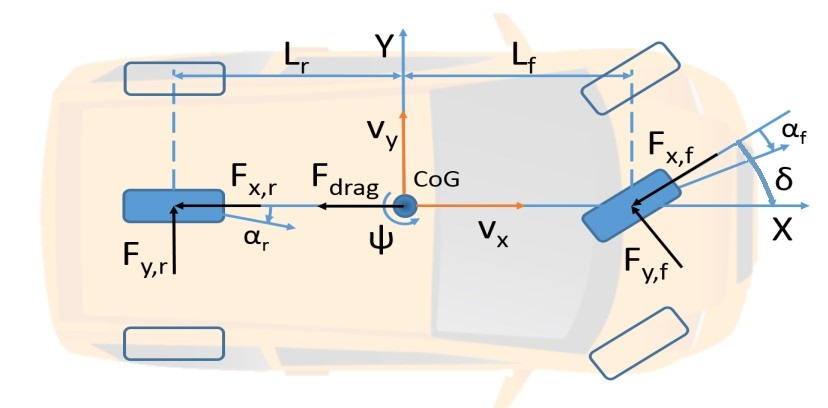
\includegraphics[width=0.5\textwidth]{Bicycle_model_paper.png}
	\caption{Non-linear bicycle model (Source: \cite{TongDuySon2019}).}
	\label{fig:bicycle_model}
\end{figure}

\section{Non-linear bicycle model}\label{sec:Vehicle_models}
The free body diagram of the non-linear bicycle model can be seen in figure \ref{fig:bicycle_model}.

Two variants of this model are discussed which are differentiated by the smoothness of the controls that are used. 
\begin{enumerate}
	\item	Model has 6 states and 2 controls: 
	\begin{equation}\label{eq:bicycle_model1}
	\centering
	\bm{X} = 
	\begin{bmatrix}
	x & y & v_x & v_y & \psi & \dot{\psi}
	\end{bmatrix}^{T}
	\; and \hspace{2mm} \; \bm{U} = 
	\begin{bmatrix}
	t_r & \delta
	\end{bmatrix}^{T}
	\end{equation}
	
	\item Model has 10 states and 2 controls:
	\begin{equation}\label{eq:bicycle_model2}
	\centering
	\bm{X} = 
	\begin{bmatrix}
	x & y & v_x & v_y & \psi & \dot{\psi} & t_r & \delta & a_x & a_y
	\end{bmatrix}^{T}
	\; and \hspace{2mm} \; \bm{U} = 
	\begin{bmatrix}
	\dot{t_r} & \dot{\delta}
	\end{bmatrix}^{T}
	\end{equation}
\end{enumerate}


$x$ and $y$ in the above formulation are the position of the centre of gravity of the vehicle in the global coordinate system. $v_x$ and $v_y$ are the vehicle velocities in the local vehicle frame. $\psi$ is the vehicle yaw angle and $\dot{\psi}$ the yaw rate. The control vector of Eq. (\ref{eq:bicycle_model1}) consists of the throttle $t_r$ and the angle of the front wheel $\delta$. In the more extended bicycle model Eq. (\ref{eq:bicycle_model2}) throttle and front wheel angle serve as states. $a_x$ and $a_y$ are the total accelerations of the centre of gravity in the local vehicle frame. The inputs in this second formulation are the first order derivatives of throttle and front wheel angle.\\

The equations of motion derived and checked in literature \cite{TongDuySon2019} are\footnote{Appendix \ref{app:A} shows the complete jerk equations $j_x$ and $j_y$.} :
\begin{equation}\label{eq:bicycle_model_eqmotion}
\begin{aligned}
\dot{x} = v_x cos(\psi) - v_y sin(\psi)\\
\dot{y} = v_x sin(\psi) + v_y cos(\psi)\\
m \dot{v}_x = F_{x,f} cos(\delta) - F_{y,f} sin(\delta) + F_{x,r} - F_{drag} + m v_y \dot{\psi}\\
m \dot{v}_y = F_{x,f} sin(\delta) + F_{y,f} cos(\delta) + F_{y,r} - m v_x \dot{\psi}\\
\dot{\psi} = \dot{\psi}\\
I_z \ddot{\psi} = L_f (F_{y,f} cos(\delta) + F_{x,f} sin(\delta)) - L_r F_{y,r}\\
\dot{t_r} = \dot{t_r}\\
\dot{\delta} = \dot{\delta}\\
a_{tx} = \dot{v}_x\\
a_{nx} = -v_y\dot{\psi}\\
a_{ty} = \dot{v}_y\\
a_{ny} = v_x\dot{\psi}\\
j_x = \dot{a}_{tx} + \dot{a}_{nx}\\
j_y = \dot{a}_{ty} + \dot{a}_{ny}
\end{aligned}
\end{equation}
\newpage
The drag force is calculated as:
\begin{equation}\label{eq:bicycle_Fdrag}
\begin{aligned}
F_{drag} = C_{r0} + C_{r1} v_x^2
\end{aligned}
\end{equation}
with $C_{r0}$ the roll resistance and $C_{r1}$ the air drag contributions.\\

To calculate the tyre forces, a linear tyre model is used instead of a more complex non-linear model e.g. Pacejka tyre model. The longitudinal tyre forces are calculated as:
\begin{equation}\label{eq:bicycle_Fx}
\begin{aligned}
F_{x,f} = \frac{t_r T_{max}}{2 R_w}\\
F_{x,r} = F_{x, f}
\end{aligned}
\end{equation}

$R_w$ is the wheel radius and $T_{max}$ the maximum torque the engine is able to supply. Because $F_{x,r} = F_{x, f}$ the longitudinal forces that are induced by the engine are equally distributed between front and rear axle (division by 2 in above equations). The coefficient $t_r$ is the normalised amount of throttle that can be applied and has a value between -1 and 1 (negative for braking). In the bicycle model it is assumed that braking behaves the same as giving a negative amount of throttle.
The lateral tyre forces are calculated based on the tyre slip angles $\alpha_f$ and $\alpha_r$:
\begin{equation}\label{eq:bicycle_slipangle}
\begin{aligned}
\alpha_f = -atan(\frac{\dot{\psi} L_f + v_y}{v_x}) + \delta\\
\alpha_r = atan(\frac{\dot{\psi} L_r - v_y}{v_x})
\end{aligned}
\end{equation}
resulting in:
\begin{equation}\label{eq:bicycle_Fy}
\begin{aligned}
F_{y,f} = 2 K_f \alpha_f\\
F_{y,r} = 2 K_r \alpha_r
\end{aligned}
\end{equation}\\
The use of this linearised lateral tyre model is valid for small lateral accelerations ($a_y <= 4 m/s^2$) and slip angles ($\alpha <= 5^o$) \cite{TongDuySon2019}. It is acceptable to use this approximate model in this thesis as the goal is to learn a comfortable and thus smooth lane change manoeuvre. However, these constraints will be checked during section \ref{s:GD_val}.\\

The vehicle model parameters used are described in table \ref{table:vehicel_model_param}. These numbers were provided by Siemens Digital Industries Software. The $Gsteerfactor$ approximates linearly the relation between the front wheel angle and the steer wheel angle turned by the driver: $\delta = \frac{\delta_s}{Gs}$.  

\begin{table}[h]
	\centering
	\begin{tabular}{|p{5cm}|p{2cm}|}
		\hline
		\textbf{Parameter} & \textbf{Value}\\ \hline	
		Vehicle mass $m$ [kg] & 1430\\ \hline
		Moment of inertia $I_z$ [$kgm^2$] & 1300\\ \hline
		Front axle distance $L_f$ [m] & 1.056\\ \hline
		Rear axle distance $L_r$ [m] & 1.344\\ \hline
		Roll resistance coefficient $C_{r0}$ [N] & 0.6\\ \hline
		Air drag coefficient $C_{r1}$ [$\frac{Ns^2}{m^2}$] & 0.1\\ \hline
		Engine torque limit $T_{max}$ [Nm] & 584\\ \hline
		Wheel radius $R_w$ [m] & 0.292\\ \hline
		Lateral front tyre stiffness $K_{f}$ [N] & 41850.85\\ \hline
		Lateral rear tyre stiffness $K_{r}$ [N] & 51175.78\\ \hline
		Gsteerfactor $Gs$ [-] &16.96 \\ \hline
		
	\end{tabular}
	\caption{Used vehicle model parameters.}
	\label{table:vehicel_model_param}
\end{table}
\newpage
\section{Learning algorithm} 
\label{s:learning_alg}
The goal of the learning algorithm is to learn the weighting factors $\bm{\theta}$ in the comfort objective function: $\bm{\theta}^T\bm{F}(\bm{r})$. It's formulation is presented in section \ref{s:flow alg}. The features that are the entries of the feature vector $\bm{F}(\bm{r})$ capture a notion of comfort felt by the driver. Based on the literature study displayed in Chapter \ref{cha:Literature_study} and on paper of Kuderer \cite{Kuderer2015a}, the amount of discomfort can be modelled by the features discussed in section \ref{s:obj} during the timespan $T$ of the maneuver. The scenario of a lane change on a straight road is modelled with the time horizon itself taken as an optimization variable $T$.


\subsection{Formulation of the algorithm}\label{s:flow alg}
%The goal of the learning algorithm is to output weighting factors that when applied in the objective $\bm{\theta}^T\bm{F}(\bm{r})$, generate feature vector  $\bm{F(\bm{r})}$ that are the best possible fit with the observed feature vector. Without a vehicle mismatch a match of feature values will directly induce a good match of the kinematic signals as is extensively discussed in section \ref{s:ID_results}. 

%This means that similarity between the observed path and the one that follows from minimizing the objective $\bm{\theta}^T\bm{F}(\bm{r})$ for chosen weighting factors, is quantified by the difference between the feature values of the observed path and the obtained one. 

As has been discussed in chapter \ref{cha:Literature_study},  $\bm{\theta}_{opti}$ gives the best possible fit between $\bm{F}(\bm{r}_{expected})$ and $\bm{\tilde{F}(\bm{r})}$.
Without a vehicle mismatch, a match of feature values will induce a good match of the kinematic vehicle signals as will be further discussed in section \ref{s:ID_results}.
The flow of a single dataset learning algorithm can be seen in Figure \ref{fig:basic learning}.\\

%The path that is expected to be produced by the driver is the path that is felt as the most comfortable and equals $\bm{r}_{expected} =  \underset{\bm{r}}{\argmin} \hspace{1mm}  \bm{\theta}^T\cdot \bm{F}(\bm{r})$.\\

The learning is started by proposing a set of weighting factors e.g. all equal to one. Equation \ref{eq:6} is minimized in order to generate an expected path. From this $\bm{F}(\bm{r}_{expected})$ can be retrieved by using the definition discussed in section \ref{s:obj}. Afterwards, the relative features $f_{rel,i}$ are calculated by element-wise  divide  the expected feature vector by the observed one $\bm{\tilde{F}}$. A perfect match is acquired when the division equals one and the learning algorithm is terminated. The tolerance on convergence towards one, is chosen during this chapter equal to $10^{-3}$.

\begin{figure}[h!]
	\centering
	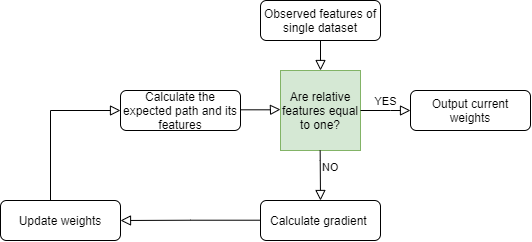
\includegraphics[width=1.0\textwidth]{basic_learning.png}
	\caption{Basic flow of the reinforced learning algorithm.}
	\label{fig:basic learning}
\end{figure}

  
While no convergence takes place the weighting factors are updated, making use of the estimation of the gradient and the RPROP algorithm explained in Chapter \ref{cha:Literature_study}. The new weighting factors are used to calculate a new expected path which will result in different expected feature values $\bm{F}(\bm{r}_{expected})$.  Next, a more detailed description of the calculation of the expected path is given by Eq. (\ref{opt:basic_opti_w}) which uses as vehicle model Eq. (\ref{eq:bicycle_model2}). \\

%In order to apply the RPROP method only the sign of the gradient is used which means that the size of the gradient is decoupled from the update value of the weighting factors. The estimate of the gradient is given by $\pdv{\bm{F}}{\bm{\theta}} = \bm{F}_{obs} - \bm{F}(\bm{r}_{expected})$  and the update of the weight is achieved by applying the gradient method according to $\bm{\theta}^{k+1} = \bm{\theta}^{k} - |\Delta \theta^{k}|sign( \pdv{\bm{F}}{\bm{\theta}}^k )$ where $\Delta \theta^{k}$ is calculated according section \ref{s:RPROP}. If follows that the weight $\theta_i$ is decreased if $f_{obs,i}>f_{i}(\bm{r_{exptected}})$ and increased when $f_{obs,i}<f_{i}(\bm{r}_{exptected})$.

\begin{equation}\label{opt:basic_opti_w}
\begin{aligned}
\min_{\bm{X}(.),\bm{U}(.), T} \quad &  \bm{\theta}^T\bm{F}(\bm{X},\bm{U}, T) \\
\textrm{s.t.} \quad & \bm{X}^{k+1} = I(\bm{X}^{k}, \bm{U}^{k}) & k = [0,\cdots, N-1]\\
& \bm{X}^{0}[1:8]= \bm{X}_{intitial} \\
& T \leq T_{limit}\\
& \bm{F}(\bm{X}^{k}) \geq 0	& k = [0,\cdots, N]\\
& \bm{H}(\bm{X}^{k}) = 0	& k = [0,\cdots, N]\\
& \bm{X}^{k}\in \mathbb{R}^{10\times 1}  & k = [0,\cdots, N]\\
& \bm{U}^{k}\in \mathbb{R}^{2\times 1} \hspace{3 mm} & k = [0,\cdots, N-1]\\
& T \in \mathbb{R},\hspace{3 mm} N \in \mathbb{N}
\end{aligned}
\end{equation}

Where $\bm{X} \in \mathbb{R}^{10\times N+1}$ and $\bm{U}\in \mathbb{R}^{2\times N}$ contain respectively the states and controls of Eq.(\ref{eq:bicycle_model2}) during the maneuver. The time of the maneuver is represented as $T$. In order to discretize time, a multiple shooting approach is adopted as explained in section \ref{s:time_dis}. The amount of integration intervals $N$ is chosen equal to $1000$ and determines the  amount of controls applied to go from the initial state towards the end state. 
Inside the function $I$ the Runge-Kutta time integration method is embedded in order to connect different states over time when a certain control is applied for $\Delta T$. Here the equations of motion Eq. (\ref{eq:bicycle_model_eqmotion}) are inputted in the optimization because derivatives of the vehicle states are needed. The time discretization used can be categorized as a direct method and because a multiple shooting approach is conducted at every time instance, a new set of state optimization variables is introduced as explained in section \ref{s:time_dis}. The path constrain vector $\bm{F}$ demarcates together with the equality constraint vector $\bm{H}$, the feasible space of the solutions for $\bm{X}$ and $\bm{U}$. An overview of the constraints used, is given by Eq. (\ref{eq:F}) and Eq. (\ref{eq:H}).

\begin{equation}\label{eq:F}
\bm{F} =
\begin{Bmatrix}
-\frac{Width\hspace{1mm}Lane}{2} \leq y^k \leq \frac{3\cdot Width\hspace{1mm}Lane}{2}, & k = [0,\cdots, N] \\
0 \leq x^k, & k = [0,\cdots, N] \\
-\frac{\pi\cdot 150}{180 Gs} \leq \delta^k \leq \frac{\pi\cdot 150}{180 Gs}, & k = [0,\cdots, N] \\
-1 \leq t_r^k \leq 1, & k = [0,\cdots, N]

\end{Bmatrix}
\end{equation}\\

\begin{equation}\label{eq:H}
\bm{H} =
\begin{Bmatrix}
y^N = Width\hspace{1mm}Lane \\ \vspace{1mm}
vy^N = 0 \\\vspace{1mm}
\psi^N = 0 \\\vspace{1mm}
\dot{\psi}^N = 0 \\\vspace{1mm}
\delta^N = 0 

\end{Bmatrix}
\end{equation}\vspace{5mm}

The constraints displayed in $\bm{H}$ make sure that at the end of the lane change, the slip angles in the tires and the steer wheel angle are zero. From Eq. (\ref{eq:bicycle_model_eqmotion}) this induces that the lateral velocity, acceleration and yaw acceleration also become zero and this marks the end of the lane change. $y^N$ ensures that the wanted lateral distance is covered. This distance can be calculated from the start position of the vehicle and the width of the lane in order to end up at the centre line of the desired lane. \\ At the start of the lane change, straight driving at constant longitudinal speed is assumed. To achieve this, the constraints of Eq. (\ref{eq:X0}) are used. No constraints for accelerations are needed. This would give a redundancy due to the other initial states in combination with the equations of motion \ref{eq:bicycle_model_eqmotion}. In Eq. (\ref{eq:X0}) all initial states are zero except the initial speed $v_{x,start}$ and $t_{r,start}$. The amount of throttle at the start of the lane change is chosen to overcome the aerodynamic drag without accelerating. This is given by $t_r^0 = \frac{(C_{r0}+C_{r1}v_{start}^2)r_w}{T_{max}}$. Therefore it can be concluded that the parameters that distinguish different lane changes are $v_{x,start}$ and $Width\hspace{1mm}Lane$. This is exploited when generating different ideal lane change datasets for chosen weighting factors. 
\newpage
\begin{equation}\label{eq:X0}
\bm{X}_{initial} =
\begin{bmatrix}
 x_{start}\\ 
 y_{start}\\
 v_{x,start}\\
 v_{y,start}\\
 \psi_{start}\\
 \dot{\psi}_{start}\\
 t_{r,start}\\
 \delta_{start}\\

\end{bmatrix}
\end{equation}


% discuss time limit is chosen equal to 25 s.
The time limit constraint in Eq. (\ref{opt:basic_opti_w}) is needed in order to demarcate the optimization solution space. When set, it has to take two conflicting criteria into account. It has to be chosen large enough in order to have a minor influence on the lane change behaviour introduced by this constraint. Secondly, it has to be taken small enough to preserve good conditions for the numerical integration performed inside $\bm{F}(\bm{X},\bm{U}, T)$, as will be seen in in \ref{s:obj}. This is because the number of optimization points $N+1$ of the states is fixed, which means that a larger time limit will give a coarser time discretization. In this thesis the time limits used are $25\hspace{1mm}s$ and $30\hspace{1mm}s$, which is a compromise between the two criteria. This choice is validated in section \ref{s:GD_val}.\\It is worth noting that with the removal of the time limit constraint the optimized comfortable lane change takes around $160 \hspace{1mm}s$. This is not a realistic results because the objective will, as previously explained, not have good numerical properties.\\ 

In order to solve Eq. (\ref{opt:basic_opti_w}) an initial guess is needed for the longitudinal velocity in order to avoid the emergence of an invalid number. The default initial guess used in the CasADi software is an all zero vector. As can be seen in Eq. (\ref{eq:bicycle_slipangle}) this would give a division by zero in the calculation of the slip angles. \\
To further enhance the solving speed of Eq. (\ref{opt:basic_opti_w}) also initial guesses are given for the other vehicle states and additionally the controls. To do this, a feasible solution of the non-linear bicycle model for a lane change is needed because IPOPT is an interior point method. Therefore, the initial guesses for $\bm{X}, \bm{U} \;and\; T$ are taken from the observed ideal data. \\

Another way to speed up the solving time of the IPOPT solver, is setting the initial guess of the lambda multipliers internally used, equal to the ones found during the previous call of Eq. (\ref{opt:basic_opti_w}) during the loop visualized by figure \ref{fig:basic learning}. \\The time needed for the CPU to calculate the expected path for a certain set of weighting factors and thus solving Eq. (\ref{opt:basic_opti_w}), takes around $5\hspace{1mm}s$ (python implementation) when a time limit of $30$ seconds and N equal to $1000$ is chosen.\\

As discussed above, the solver used to calculate the states and control signals in Eq. (\ref{opt:basic_opti_w}), is IPOPT which is an open source solver. The idea behind it is to smoothing the KKT conditions and transform it into a smooth root finding problem. \cite{Panos_opti} \\

%Because IPOPT is a interior boundary method, a feasible initial guess is needed.
% Every time that the expected path has to be calculated as is visualised in flow diagram \ref{fig:basic learning}, the optimization \ref{opt:basic_opti_w} is performed with as initial guess the observed maneuver.\\

\subsection{Objective function}\label{s:obj}
The objective function used in Eq. (\ref{opt:basic_opti_w}) has to represent comfort felt by the driver and is based on the literature study displayed in section \ref{s:comfort_parameters}. The choice made in how to define the different features is important because it sets the fixed framework where the weighting factors will be learned in.  It can be expected that the linear relation of features given by $\bm{\theta}^T\bm{F}(\bm{r})$ will serve as an approximation for the real, more complex comfort objective of a human drive. The feature framework that is further discussed in this section, can be validated and adjusted based on an user study.\\

%As is showed in \cite this linear approximation of features can already capture  the main trends that contribute to an comfortable maneuver experience.

\begin{equation}\label{eq:obj}
discomfort = \theta_1 \cdot f_1 +\theta_2 \cdot f_2 +\theta_3 \cdot f_3 +\theta_4 \cdot f_4 +\theta_5 \cdot f_5 +\theta_6 \cdot f_6 \\
\end{equation}
\[	f_i, \theta_i \in \mathbb{R} \hspace{5mm}
i \in \mathbb{N}\]


\textit{Feature 1: longitudinal acceleration}
\begin{equation}\label{eq:flong_acc}
f_{1}:\bm{r}\xrightarrow{}f_1(\bm{r})=\int_{0}^{T}a_{x,total}^{2}(t) dt
\end{equation}
Feature one is assessing the amount of discomfort by integrating the total longitudinal acceleration in the local axis. The local axis is fixed to the centre of gravity of the vehicle, as can be seen in Figure \ref{fig:bicycle_model}. The total longitudinal acceleration  $a_{x,total} $ is the sum of  $ a_{x,tangential}$ and $a_{x,normal}$ as described in Eq. (\ref{eq:bicycle_model_eqmotion}). \\

\textit{Feature 2: lateral acceleration}
\begin{equation}\label{eq:flat_acc}
f_{2}:\bm{r}\xrightarrow{}f_2(\bm{r})=\int_{0}^{T}a_{y,total}^{2}(t) dt
\end{equation}
Feature two is assessing the amount of discomfort by integrating the total lateral acceleration in the local axis. The total lateral acceleration  $a_{y,total} $ is the sum of  $ a_{x,tangential}$ and $a_{x,normal}$ as described in Eq. (\ref{eq:bicycle_model_eqmotion}).\\

\textit{Feature 3: longitudinal jerk}
\begin{equation}\label{eq:flong_jerk}
f_{3}:\bm{r}\xrightarrow{}f_3(\bm{r})=\int_{0}^{T}j_{x}^{2}(t) dt
\end{equation}
Feature three is giving the amount of comfort by integrating the total change of longitudinal acceleration during the followed path. \\

\textit{Feature 4: lateral jerk}
\begin{equation}\label{eq:flat_jerk}
f_{4}:\bm{r}\xrightarrow{}f_4(\bm{r})=\int_{0}^{T}j_y^{2}(t) dt
\end{equation}
Feature four is given the amount of comfort by integrating the total change of lateral acceleration during the followed path. \\

\textit{Feature 5: desired speed}
\begin{equation}\label{eq:des_speed}
f_{5}:\bm{r}\xrightarrow{}f_5(\bm{r})=\int_{0}^{T}(v_{des}-v_x)^2 dt
\end{equation}
$v_{des}$ is assumed to be a constant value and set equal to the start velocity just before the lane change.\\

\textit{Feature 6: desired lane change}
\begin{equation}\label{eq:des_lane_change}
f_{6}:\bm{r}\xrightarrow{}f_6(\bm{r})=\int_{0}^{T}(L-y)^2 dt
\end{equation}

$L$ is a constant and set equal to the desired lateral distance. If the vehicle reaches its desired lateral displacement faster, this is perceived as a good response and is interpreted as comfort as is discussed in section \ref{s:comfort_parameters}.\\

In order to implement the above defined integrals in the objective function of Eq. (\ref{opt:basic_opti_w}), discretization is needed. For this the Crank-Nicolson numerical integration is used as is shown in Eq. (\ref{eq:CN}) for feature $f_j$. 
\begin{subequations}\label{eq:CN}
	\begin{equation}
	\int_{f_j(t^n)}^{f_j(t^{n+1})}df_j=\int_{t^n}^{t^{n+1}} P(t) \cdot dt	
	\end{equation}
	\begin{equation}
	f_j^{n+1} -f_j^{n} = \frac{1}{2}\frac{P(t^{n+1})+P(t^n)}{\Delta T}
	\end{equation}
\end{subequations}\\

To summarize, the objective described by Eq. (\ref{eq:obj}) consists out of a set of comfort features that model the amount of discomfort experienced during a maneuver. This is achieved by mapping kinematic signals onto scalar feature values through integration. By finding the driver specific weighting factors $\bm{\theta}$ in Eq. (\ref{eq:obj}), it is possible to model driver preferences between different comfort features. With this information an autonomous vehicle can perform path planning of the most comfortable path to do a lane change for a specific driver.\\

As is shortly discussed in Chapter \ref{cha:Literature_study}, the perception of save driving contributes to the amount of comfort that is experienced. Save driving comprises next to smooth behaviour also distances between other road agents. However features that consider the environment are not taken into account in Eq. (\ref{eq:obj}). This can be done if data of the position of other vehicles during the maneuver is available. Paper \cite{Kuderer2015a} gives some suggestions showed by Eq. (\ref{eq:comfort_feature}) and  Eq. (\ref{eq:lane_d}).  
\newpage

\begin{equation}\label{eq:comfort_feature}
f_d= \sum_{k = 1}^{NA}\int_{0}^{T}\frac{1}{(x_{o,k}(t)-x)^2+(y_{o,k}(t)-y)^2}\cdot dt
\end{equation}
\[L \in \mathbb{N}\]

With $[x_o,y_o]_k$ the position of the closest point of a different agent and $NA$ the total amount of road agents in the nearby area.\\

Not only the bird's eye view distance between two different vehicles plays a role, also the following distance of vehicle in the same lane is important. This can be modelled as:  

\begin{equation}\label{eq:lane_d}
f_d= \int_{0}^{T} max(0,\hat{d}-d(t))\cdot dt
\end{equation}


The minimum desired following distance $\hat{d}$ can be calculated based on the  distance needed to avoid collision during unexpected events when driving at a certain longitudinal velocity. \\

An other assumption that is not discussed in this thesis is the time limit to finish a maneuver. In a real life application however, this limit often influences the maneuver. After the weighting factors are identified, the most comfortable path with a constraint time horizon can be planned for a specific driver. 

\subsection{Normalization factors} \label{s:norm}
To reduce the effect of order of magnitude given by the units in the objective, a normalization of the features is done. The kinematic signals of an example lane change are produced and the same features that are used in the objective function are calculated from it. These will be the normalization factors as can be seen in Eq. (\ref{eq:obj_ideal_data}). Table \ref{table:norm} gives an overview of the lane change normalization factors used.  % hoe ook al weer gegenereerd? 

%The longitudinal jerk normalization factor is taken equal to the one used for the longitudinal acceleration.
%Then the objective function is divided by the corresponding normalization factor which means that a feature that inherently gives a small feature value, will be divided by a small value and the other way around, an inherently large feature value will be divided by a large value.

%$ \bigl[ \begin{smallmatrix} 4,&5,&6,&1,&2\end{smallmatrix}\bigr]$
\begin{table}[h!]
  \centering
  \begin{tabular}{@{}lr@{}} 
    Normalization factor    & Value\\ \midrule
    Nr.1      & 0.0073\\
    Nr.2          & 2.64\\
    Nr.3 	   & 0.0073\\
    Nr.4       & 11.28\\
    Nr.5       & 0.047\\
    Nr.6  & 17.14\\ \bottomrule
  \end{tabular}
  \caption{Overview of  normalization factors.}
  \label{table:norm}
\end{table}

Because of the normalization the relative weighting factors defined as $\theta_{r,i} = \frac{\theta_{abs,i}}{norm_i}$, will quantify the trade-offs between different comfort features without disturbance of units used. Aside of this it allows to learn weighting factors faster, because of the absence of big size differences induced by unit differences that are present in the absolute weighting factors. During the learning loop (Figure \ref{fig:basic learning}) the max weight update is set to a maximum of $1$ in this thesis. When the absolute weighting factors are learned instead of the relative ones, this would give a substantially higher amount of iterations when started from an initial guess an all-one vector.

\section{Ideal data} \label{s:GD}
As mentioned at the begin of this chapter the term 'ideal data' concerns data that is generated with a non-linear bicycle model and with a beforehand known objective function Eq. (\ref{eq:obj}) which consist out of a linear combination of features and weighting factors $\bm{\theta}$. This means that the algorithm that learns the weighting factors can be validated by checking if it is able to find back the correct weighting factors. First the generation of ideal data is presented in section \ref{s:generation} whereafter it is validated in section \ref{s:GD_val}.

\subsection{Generation}
\label{s:generation}
The relative weighting factors chosen to generate the data are $ \bigl[ \begin{smallmatrix} 4,&5,&1,&6,&1,&2\end{smallmatrix}\bigr]$, which gives as absolute weighting factors  $ \bigl[ \begin{smallmatrix} 549.75, &1.90, &137.44  ,&0.53,  &21.43, &0.12\end{smallmatrix}\bigr]$ when the normalization discussed in section \ref{s:norm} is taken into account. The objective that is used in Eq. (\ref{opt:basic_opti_w}) is given by Eq. (\ref{eq:obj_ideal_data}). The different feature values are the ones as defined in section \ref{s:obj}.

\begin{equation}\label{eq:obj_ideal_data}
\frac{4}{0.0073} \cdot f_1 +\frac{5}{2.64} \cdot f_2 +\frac{1}{0.0073} \cdot f_3 +\frac{6}{11.28} \cdot f_4 +\frac{1}{0.047} \cdot f_5 +\frac{2}{17.14} \cdot f_6 
\end{equation}
\[	f_i \in \mathbb{R}, \hspace{1mm}
i \in \mathbb{N}\]

 When multiple ideal datasets have to be generated in order to serve as observations, the initial speed $V_{0}$ and width of the lateral distance $L$ are varied.

\subsection{Validation} \label{s:GD_val}
In this section the results of the generated ideal data are discussed. There is being look at an numerical vs analytical formulation, influence of the initial guess, choice of time limit, amount of control points, use of linear tire model and a discussion on the resulting feature values of the generated data.

\subsubsection{Numerical vs Analytical formulation}
In section \ref{sec:Vehicle_models} about the non-linear bicycle model, two different variants were described by Eq. (\ref{eq:bicycle_model1}) and Eq. (\ref{eq:bicycle_model2}). Variant one has only 6 states and the accelerations and jerks in the objective function Eq. (\ref{eq:obj}) are calculated by making use of numerical differentiation described by Eq. (\ref{eq:diff}) from the other vehicle states. Variant two on the other hand has the total accelerations as direct states in the vehicle model and uses an analytical formulation of the jerk described in appendix \ref{app:A}.

\begin{subequations}\label{eq:diff}
	\begin{equation}
	\pdv{\phi}{t} = \frac{\phi(i+1)-\phi(i-1)}{2\Delta t}
	\end{equation}
	\begin{equation}
	\pdv[2]{\phi}{t} = \frac{\phi(i+1)-2\phi(i)+\phi(i-1)}{\Delta t^2}
	\end{equation}
\end{subequations}

In order to validate the two approaches the generated lateral jerk signals are compared in Figure \ref{fig:comp_jerks}.

\begin{figure}[h!]
	\centering
	\begin{minipage}{.5\textwidth}
		\centering
		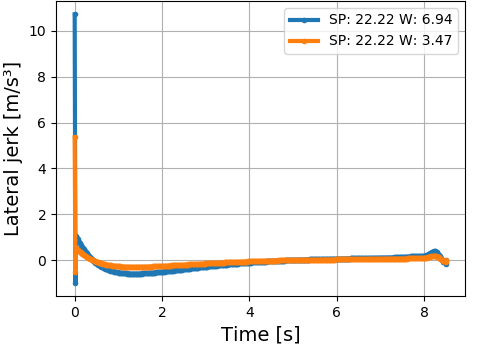
\includegraphics[width=1.0\linewidth]{jerk_num.png}
		%		\captionof{figure}{Lateral jerk using \ref{eq:diff}.}	
	\end{minipage}%
	\begin{minipage}{.5\textwidth}
		\centering
		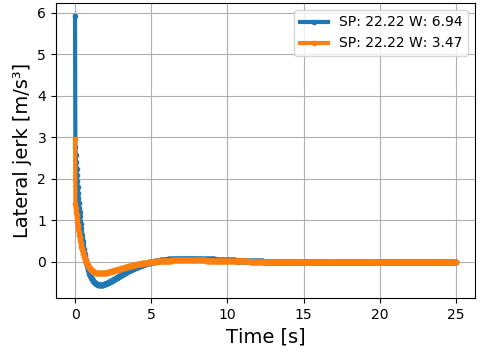
\includegraphics[width=1.0\linewidth]{jerk_ana.png}
		%		\captionof{figure}{Lateral jerk using appendix \ref{app:A} .}	
	\end{minipage}
	\caption{A comparison between the numerical jerk (left) based on Eq. (\ref{eq:diff}) and Eq. (\ref{eq:bicycle_model1}) and the analytical jerk (right) based on appendix \ref{app:A} and Eq. (\ref{eq:bicycle_model2}). }
	\label{fig:comp_jerks}
\end{figure}

It is clear that the analytical formulation (right figure)  of the jerk gives more smooth results and less high peaks which is in line with observations of the more complex $15$ dof Amesim vehicle that is discussed in chapter \ref{cha:Tracking_MPC}. Therefore the analytical formulation approaches reality better. An other way to see this is that the analytical formulation contains more information about the vehicle i.e. the equations resulting from numerical differentiation are approximations of the analytical ones.

\subsubsection{Initial guess}
To determine if the generated data is a local solution, two different initial guesses $V0:22.22 - L3.47$ and $V0:25.00 - L6.94$ are used whereof the retrieved data feature values are summarized in table \ref{tab:GD_local_test}. $V_0$ is the initial speed and $L$ the lateral distance of the lane change used as initial guess and are generated using the above described numerical formulation. In order to calculate the data features displayed, time limit is set on $30\hspace{1mm}s$, N on $1000$, $V_{0} = 22.22\hspace{1mm}\frac{m}{s}$ and $L = 3.47\hspace{1mm}m$ as parameters in Eq. (\ref{opt:basic_opti_w}) and the analytical formulation is used. From the results it is suggested that the generated data feature values are not a local solution because they are found back from different start points of the optimization. During the learning of the weighting factors as described in Figure \ref{fig:basic learning} the initial guess is set equal to the observed data. 

\begin{table}[h!]
	\centering
	\begin{tabular}{@{}llr@{}} \toprule
		\textbf{Feature Value}     & V0:22.22 - L3.47 & V0:25.00 - L6.94\\ \midrule
		Nr.1       & 6.83e-8   & 6.83e-8 \\
		Nr.2       & 0.37        & 0.37  \\
		Nr.3       & 1.77e-7     & 1.77e-7 \\
		Nr.4       & 0.57    & 0.57  \\
		Nr.5       & 1.98e-6     & 1.98e-6 \\
		Nr.6       & 30.94      & 30.94\\ \bottomrule
	\end{tabular}
	\caption{This table shows the retrieved feature values using the two different  initial guesses in Eq. (\ref{opt:basic_opti_w}).}
	\label{tab:GD_local_test}
\end{table}

\subsubsection{Time limit}
In order to check the dependency of the generated data on the chosen $T_{limit}$ constraint in Eq. (\ref{opt:basic_opti_w}), data is generated for a lane change with N, the amount of control points equal to $1000$, initial velocity equal to $80 \hspace{1 mm} \frac{km}{h}\hspace{1mm}(V_{0})$, a desired lateral displacement of $3.47\hspace{1mm}m\hspace{1mm}(L)$ and a varying $T_{limit}$ constraint as indicated in table \ref{tab:GD_time_limit}. Figures that  show what the difference in feature values actually means for the different kinematic signals of the vehicle, can be consulted in Appendix \ref{app:B}.

\begin{table}[h!]
	\centering
	\begin{tabular}{@{}llllr@{}} \toprule
		\textbf{Feature Value}    & 20 s  & 50 s      & 100 s\\ \midrule
		Nr.1       & 3.66e-8     & 1.13e-7   & 2.04e-7\\
		Nr.2       & 0.37        & 0.38      & 0.38\\
		Nr.3       & 1.13e-7     & 3.98e-7   & 1.56e-6 \\
		Nr.4       & 0.58        & 0.57      & 0.54\\
		Nr.5       & 1.72e-6     & 2.27e-6   & 3.16e-6\\
		Nr.6       & 31.05       & 30.74     & 30.42\\ \bottomrule
	\end{tabular}
	\caption{This table shows the retrieved feature values using different time limits in Eq. (\ref{opt:basic_opti_w}).}
	\label{tab:GD_time_limit}
\end{table}
Looking at even greater time limits is not desirable because beyond a time limit of $100 \hspace{1mm}s$, the time discretization gets larger than $0.1\hspace{1mm}s$ for N equal to $1000$ which will result in an more unreliable discretization.\\

From the result of table \ref{tab:GD_time_limit} it can be concluded that the influence of the manually setting of the time limit in Eq. (\ref{opt:basic_opti_w}), can be neglected. The lateral features that are the most important ones as will be discussed in section \ref{s:fv_val} are very similar and also the kinematic signals for the lateral variables found in Appendix \ref{app:B} show the same behaviour.

\subsubsection{Amount of control points}
The test carried out to investigate the dependence of the resulting feature values on the amount of control points $N$, uses the same parameters as described in the previous section but fixes the time limit on $30\hspace{1mm}s$ and varies N over $500$, $1000$ and $1500$ points. The results are shown in table \ref{tab:GD_N} whereof it follows that a choice of N equal to $1000$ is justified considering the small difference of the obtained features when N is chosen equal to $1500$. For a full overview of the different kinematic signals, reference is made to Appendix \ref{app:B}. Again the kinematic vehicle signals confirm the same conclusion as taken from table \ref{tab:GD_N}.

\begin{table}[h!]
	\centering
	\begin{tabular}{@{}llllr@{}} \toprule
		\textbf{Feature Value}    & 500   & 1000       & 1500 \\ \midrule
		Nr.1       & 9.42e-8     & 6.63e-8   & 6.45e-8\\
		Nr.2       & 0.38        & 0.37      & 0.37\\
		Nr.3       & 5.61e-7     & 1.77e-7   & 1.11e-7 \\
		Nr.4       & 0.56        & 0.57      & 0.58\\
		Nr.5       & 2.50e-6     & 1.98e-6   & 1.85e-6\\
		Nr.6       & 30.66       & 30.94     & 31.05\\ \bottomrule
	\end{tabular}
	\caption{This table shows the retrieved feature values using different amount of control point N in Eq. (\ref{opt:basic_opti_w}).}
	\label{tab:GD_N}
\end{table}


\subsubsection{Linear tire model}
In this section it is checked if the conditions to use a linearised lateral tire model is valid. In literature \cite{TongDuySon2019} it was found that this is the case when there are small lateral accelerations ($a_y <= 4 \frac{m}{s^2}$) and slip angles ($\alpha <= 5^o $) during the maneuver. Figure \ref{fig:lat} gives the total lateral acceleration during a lane change maneuver that moves two lanes or an estimated lateral distance of $6.94 m$. Figure \ref{fig:slip} shows the slip angle during this maneuver. From the graphs it can be concluded that the linearisation of the lateral tire forces is valid and there is no need for a more complex tyre model embedded in Eq. (\ref{opt:basic_opti_w}).  Both figures are generated with the complex vehicle model discussed in chapter \ref{cha:Tracking_MPC} and make use of Eq. \ref{eq:bicycle_slipangle} in order to estimate the slip angle.

 \begin{figure}[h!]
	\centering
	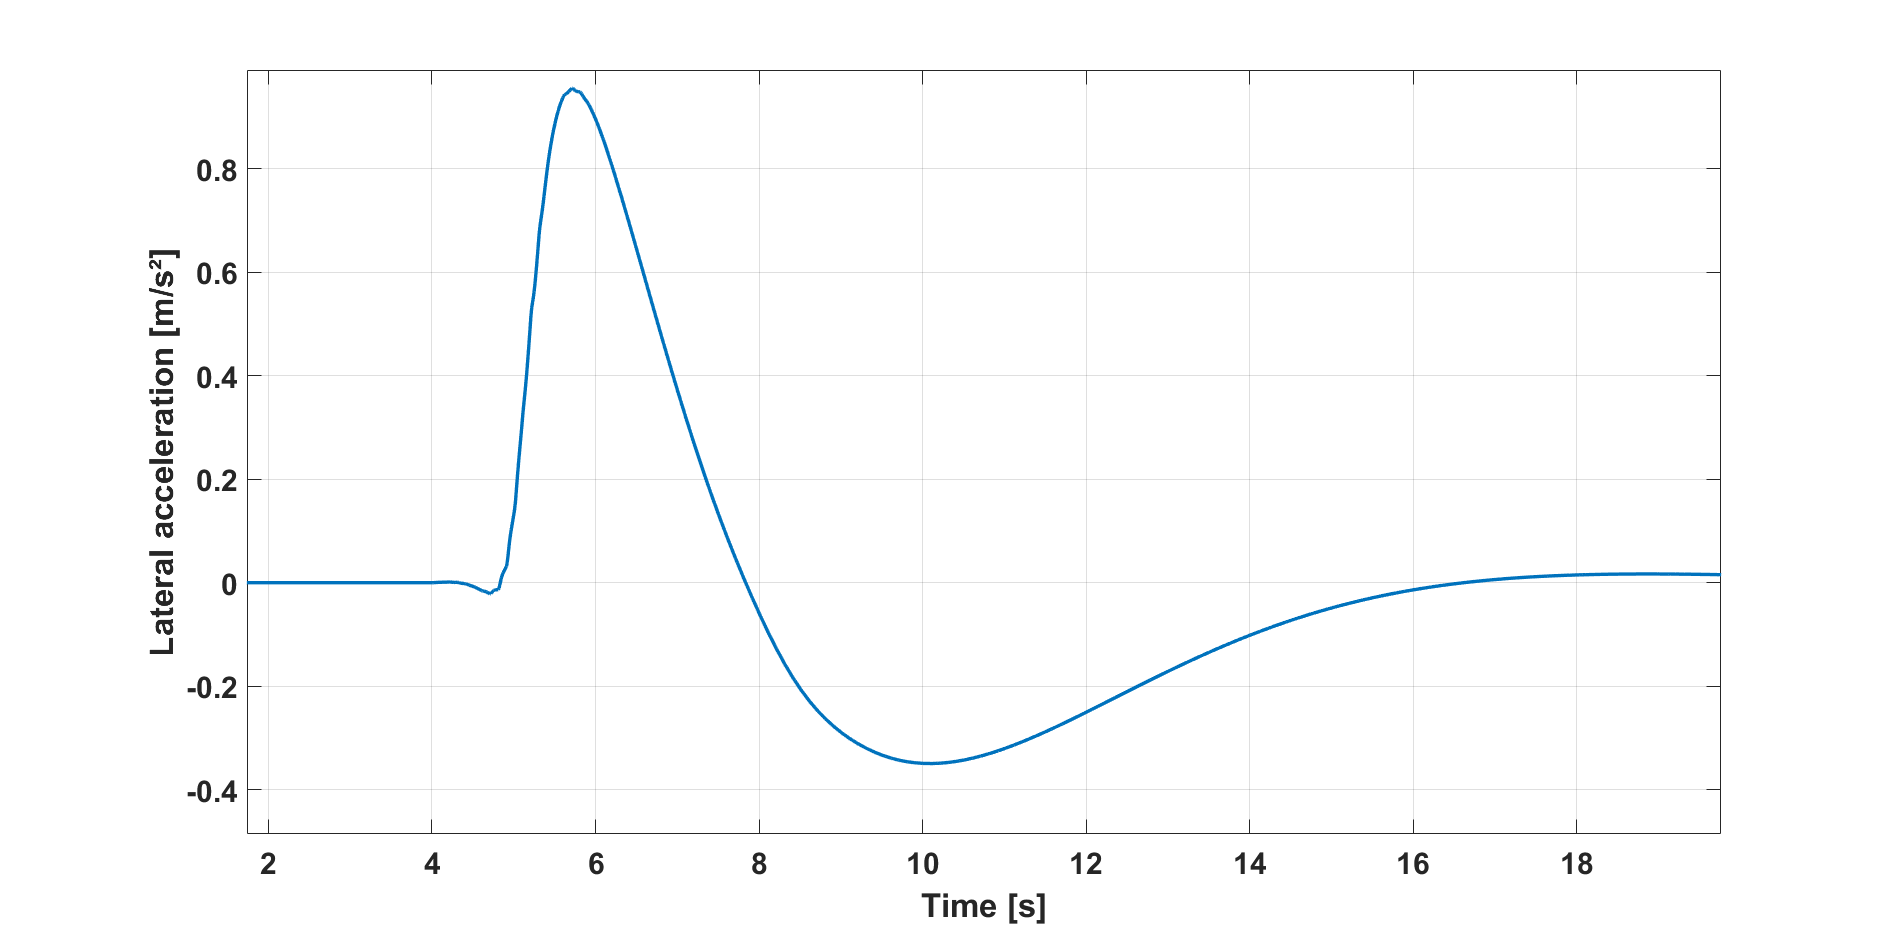
\includegraphics[width=1.0\textwidth]{lat_acc.png}
	\caption{Lateral acceleration during a lane change $V_0: 25.00 \frac{m}{s}$ and $L:6.94 m$ generated with the $15$ dof Amesim model.}
	\label{fig:lat}
\end{figure}

 \begin{figure}[h!]
	\centering
	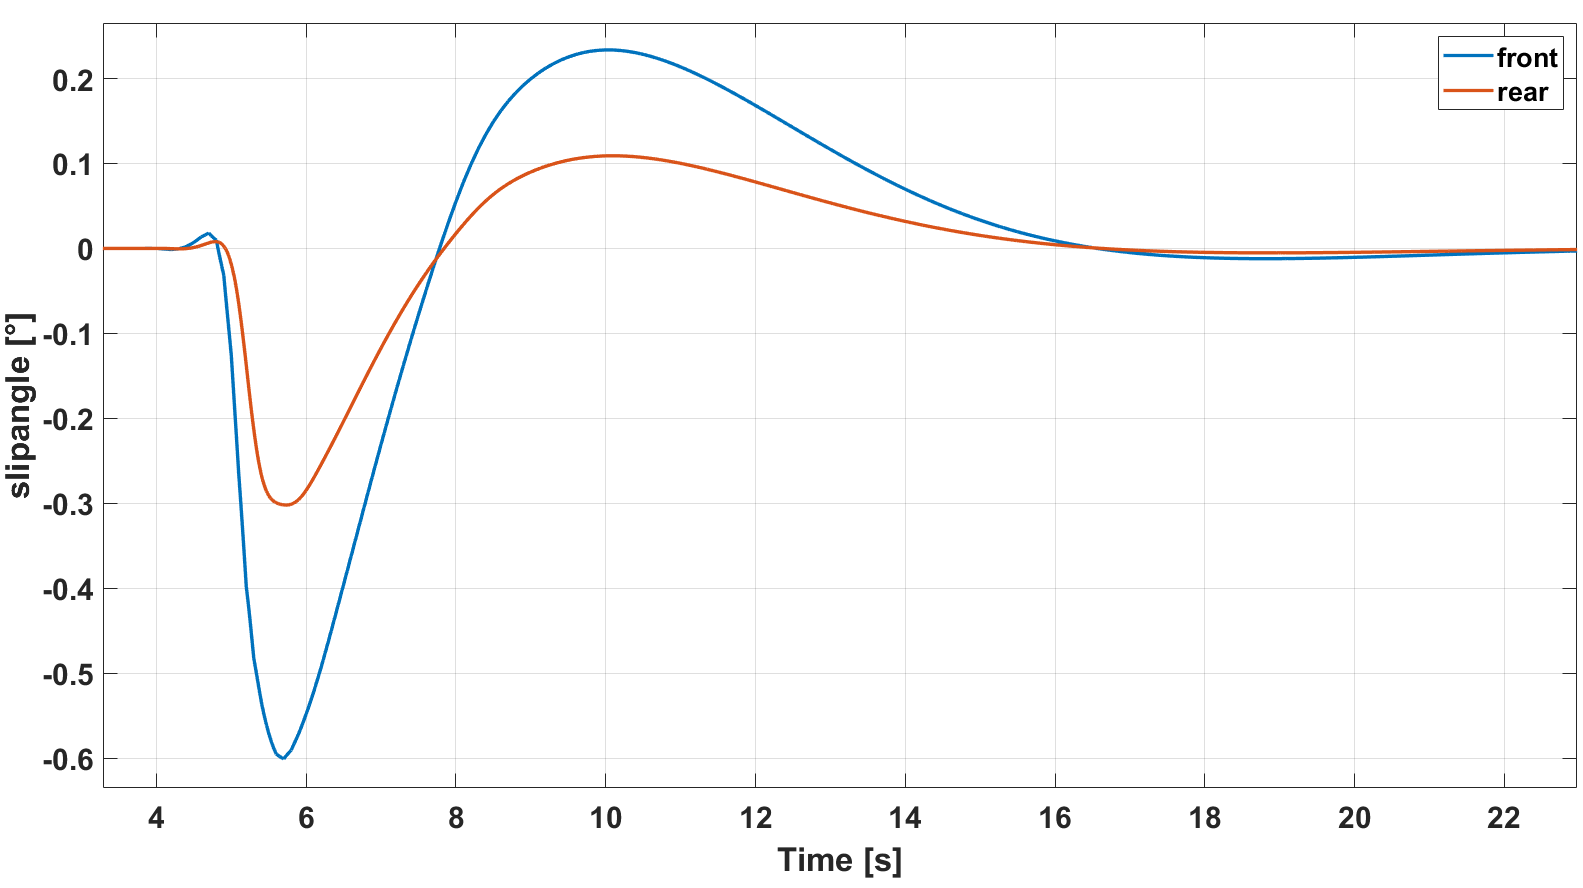
\includegraphics[width=1.0\textwidth]{slipangle_V25.00-L6.94-amesim.png}
	\caption{slip angle during lane change $V_0: 25.00 \frac{m}{s}$ and $L:6.94 m$ generated with the $15$ dof Amesim model.(blue:front,red:rear)}
	\label{fig:slip}
\end{figure}


\subsubsection{Feature values} \label{s:fv_val}
% Steeds dezelfde als enkel horizontale init speed verandert --> zelfde gewichten zullen geleerd worden aangezien enkel de lateral featues bijdragen. 
In the above tables it can be seen that the first, third and fifth feature values concerning longitudinal behaviour of the vehicle are very small. This often means that during a lane change these features have a low influence. It can be expected that for small observed feature values, it becomes hard to accurately learn weighting factors that generate feature values that match with these small values. The reason for this is because the feature value is negligible which means that any weight times zero stays zero in the objective function of Eq. \ref{opt:basic_opti_w}. For this reason almost any weight can be used for the longitudinal features without observing a different lane change outputted by the optimization done in Eq. \ref{opt:basic_opti_w}. This will be further discussed in section \ref{s:SDL}.\\% A suggested solution for this is the use of different features or an different maneuver. Scaling in the calculation of the gradient doesn't help. RPROP update is independent of the order of size of the gradient. 

An other interesting observation about the generated data features is that when the initial speed of the lane change is varied and the desired lateral displacement stays the same, because of the small longitudinal feature values the data features found are almost identical. 

\subsubsection{Conclusion}
In this section there has been looked into the correctness of the generated data making use of Eq. (\ref{eq:bicycle_model2}), that further will be used to learn from. The influence of different choices i.e. initial guess, the time limit and the amount of control points has been checked. Out of this it followed that the same data features were found for different intial guesses and it is allowed to take the time limit equal to $30 \hspace{1mm}s$ and the amount of control points to $1000$ as is done further on in this thesis. Next it has been shown that it is justified to use a linearised tire model. Finally the resulting feature values of the ideal data were shortly look into. It was concluded that a worse learning is expected for the retrieved longitudinal features due to their small values. 

\section{Ideal data learning results} \label{s:ID_results}
In this section the results of learning weighting factors from ideal data is discussed.
Section \ref{s:SDL} concerns the learning of a single dataset $V_0:22.22\hspace{1mm}\frac{m}{s},\hspace{1mm} L:3.47\hspace{1mm}m$. In reality one demonstrated demonstration doesn't capture perfectly the preference of a human driver. In order to do so, learning of multiple datasets is needed. Therefore the averaging method is presented in section \ref{s:averaging_method} and the conflict method in section \ref{s:conflict_method}. Afterwards a comparison is made in section \ref{s:comparison of methods}.\\

It is known beforehand that the weighting factors used to generate the data feature values are  $\bigl[ \begin{smallmatrix} 4,&5,&1,&6,&1,&2\end{smallmatrix}\bigr]$\footnote{The corresponding features  of the chosen weighting factors can be seen in section \ref{s:obj} and are summarized by $\bigl[ \begin{smallmatrix} f_{ax},&f_{ay},&f_{jx},&f_{jy},&f_{diff vx},&f_{diff y}\end{smallmatrix}\bigr]$.} and the initial guess of the weighting factors is chosen as an all-one vector. The convergence criteria to stop the learning loop as displayed in Figure \ref{fig:basic learning}, is when the maximum amount of iterations set to $300$ is reached or if the data feature values are accurately regenerated with learned weighting factors.\\
This is quantified by $f_{rel,i} = \frac{f_{learned,i}}{f_{obs,i}} \leq 10^{-3}$.  $\bm{f}_{obs}$ equals the generated data feature vector retrieved according to section \ref{s:GD} and is constant during learning. $\bm{f}_{learned}$ is the feature vector calculated from the learned path and changes during every learning loop. Convergence is reached when the three lateral feature values $2$, $4$ and $6$, that dominantly define the lane change, are accurately fitted for a certain set of weighting factors. The simulations done in this thesis are performed on a notebook provided by Siemens with Intel Core i7-7920HQ CPU @ 3.10GHz and 32 GB of RAM memory.\\
		
\subsection{Single dataset learning}\label{s:SDL}
The generated data features that have to be matched, can be seen in table \ref{tab:GD_local_test}.
The resulting weight vector $\bm{\theta}$ and $\bm{f}_{rel}$ outputted at convergence on iteration $28$ is displayed in table \ref{tab:comp_it}. The weight concerning the lateral acceleration (Nr.$2$) is taken as reference in order to compare the learned weighting factors with the chosen ones. The results show that the lateral weighting factors are found accurately back. Table \ref{tab:comp_it} also shows the results when the algorithm is manually set to run for $121$ iterations.
A clear difference between the lateral features that have an increased matching of $f_{rel,i}$ with an accuracy of $10^{-6}$ is seen. The convergence of the longitudinal features $f_{rel,i}$ towards one, didn't increase much because they are constraint in the accuracy that they can be learned. 

\begin{table}[h!]
	\centering
	\begin{tabular}{@{}llllr@{}} \toprule
					      & $It.28-\bm{\theta}$ & $It.28-\bm{f_{rel}}$ & $It.121- \bm{\theta}$ & $It.121-\bm{f_{rel}}$\\ \midrule
		Nr.1       		  &14.469        & 0.9907 	    & 10.021 &	1.0004	\\
		Nr.2              &5.000       & 0.9995       & 5.000 &   1.0000   \\
		Nr.3              & 3.045       & 1.0037       & 2.179 &  0.9976    \\
		Nr.4              & 5.977       & 1.0006       & 5.998 & 1.0000     \\
		Nr.5              & 3.689       & 0.9941       & 2.538 &   0.9892   \\
		Nr.6              & 1.998       & 1.0001       & 2.002 &  1.0000    \\ \bottomrule
	\end{tabular}
	\caption{This table shows the weighting factors learned from the dataset $V_0:22.22\frac{m}{s}-L:3.47m$ and the associated $\bm{f}_{rel}$ at a two different amount of iterations.}
	\label{tab:comp_it}
\end{table} 

 As already suggested in section \ref{s:fv_val} this is because of the small size of the feature values of the longitudinal direction. Not very accurate learned longitudinal feature values will have a negligible influence on the overall behaviour of the planned path and as can be seen, a range of weighting factors will give an acceptable match quantified by $f_{rel,i}$.\\
 In order to learn the longitudinal weighting factors of the human driver accurately, a maneuver should be considered were these features will be more prominent e.g. an acceleration maneuver or different features can be chosen e.g. $a_{tot}^2 = a_x^2 + a_y^2$. Because the interest in the longitudinal weighting factors during a lane change is marginal this is not further discussed during this thesis.\\          

It could be argued that if the longitudinal feature weighting factors are not so important in defining the lane change, they have to be removed from the objective Eq. (\ref{eq:obj}). This is however not an correct assumption. The longitudinal features are less dominant during a lane change and therefore different longitudinal weighting factors give rise to the same lane changes. However, they still play a roll in comfortable path planning in order to avoid nervous throttle and consequently longitudinal jerk and acceleration behaviour. 


\subsection{Averaging method}\label{s:averaging_method}
In order to simultaneously learn from multiple datasets the averaging method is proposed. \cite{Kuderer2015a} The flow of the algorithm is similar as shown in Figure \ref{fig:basic learning} and the convergence criteria stays the same $f_{rel,i} = \frac{f_{learned,i}}{f_{obs,i}} \leq 10^{-3}$. However, instead of inputting a data feature vector $\bm{f}_{obs}$ based on a single dataset, an averaged one over multiple datasets is used.\\
To calculate the gradient used to update the weighting factors $\bm{\theta}$, the difference between the averaged data feature vector and the averaged learned feature vector is taken. In order to obtain the averaged learned feature vector, $m$ times the optimization Eq. (\ref{opt:basic_opti_w}) is called with $m$ the amount of observed maneuvers. After solving the $m$ resulting learned feature vectors they are averaged. Each distinct maneuver has a different initial longitudinal speed and desired lateral displacement.\\
 
 % Bespreek de fixed feature approach.

The datasets chosen to perform the learning on are: $V_0:22.22\hspace{1mm}\frac{m}{s}-\hspace{1mm} L:3.47\hspace{1mm}m$, $V_0:25.00\hspace{1mm}\frac{m}{s}-\hspace{1mm} L:3.47\hspace{1mm}m$ and $V_0:22.22\hspace{1mm}\frac{m}{s}-\hspace{1mm} L:6.94\hspace{1mm}m$. The resulting weighting factors and average $\bm{f}_{rel}$ found after $25$ iterations are respectively $\bigl[ \begin{smallmatrix} 14.459,&5.000,&3.204,&5.984,&3.720,&2.000\end{smallmatrix}\bigr]$ and $\bigl[ \begin{smallmatrix} 0.9981,&0.9996,&0.9829,&1.0000,&0.9946,&1.0001\end{smallmatrix}\bigr]$. This means that the lateral chosen weighting factors are accurately found back. The $\bm{f}_{rel}$ of the individual datasets can be seen in table \ref{tab:in_av}.  The individual $\bm{f}_{rel,i}$ at convergence shows how good the match of feature values is when applying the learned weighting factors at Eq. (\ref{opt:basic_opti_w}) with the same parameters for $V_0$ and $L$. It is shown that there is a good match between the learned feature vectors and the individual data feature vectors.
 
\begin{table}[h!]
	\centering
	\begin{tabular}{@{}llllr@{}} \toprule
		\textbf{Feature}    & V022.22 - L3.47 & V022.22 - L6.94 & V025.00 - L3.47\\ \midrule
		Nr.1       		  &1.0000        & 0.9973 	    & 1.0064 		\\
		Nr.2              & 1.0002       & 0.9992       & 1.0001       \\
		Nr.3              & 0.9860       & 0.9816       & 0.9983       \\
		Nr.4              & 1.0012       & 0.9995       & 1.0010       \\
		Nr.5              & 0.9972       & 0.9948       & 0.9902       \\
		Nr.6              & 0.9999       & 1.0002       & 0.9999       \\ \bottomrule
	\end{tabular}
	\caption{This table shows the $\bm{f}_{rel}$ for each individual dataset at convergence using the average method.}
	\label{tab:in_av}
\end{table} 
Figure \ref{fig:3D_learned_path} shows the three initial guesses of the paths that make use of an all-one weight vector in red, purple and brown. The finally learned paths can be seen in pink, grey and yellow. These paths lay exactly on the observed ones. From this it is concluded that matching of feature values which are scalars, give a good representation for the matching performance of the 2D kinematic vehicle signals. The rest of the kinematic signals originating from the non-linear bicycle model can be seen in Appendix \ref{app:C}. 

 \begin{figure}[h!]
	\centering
	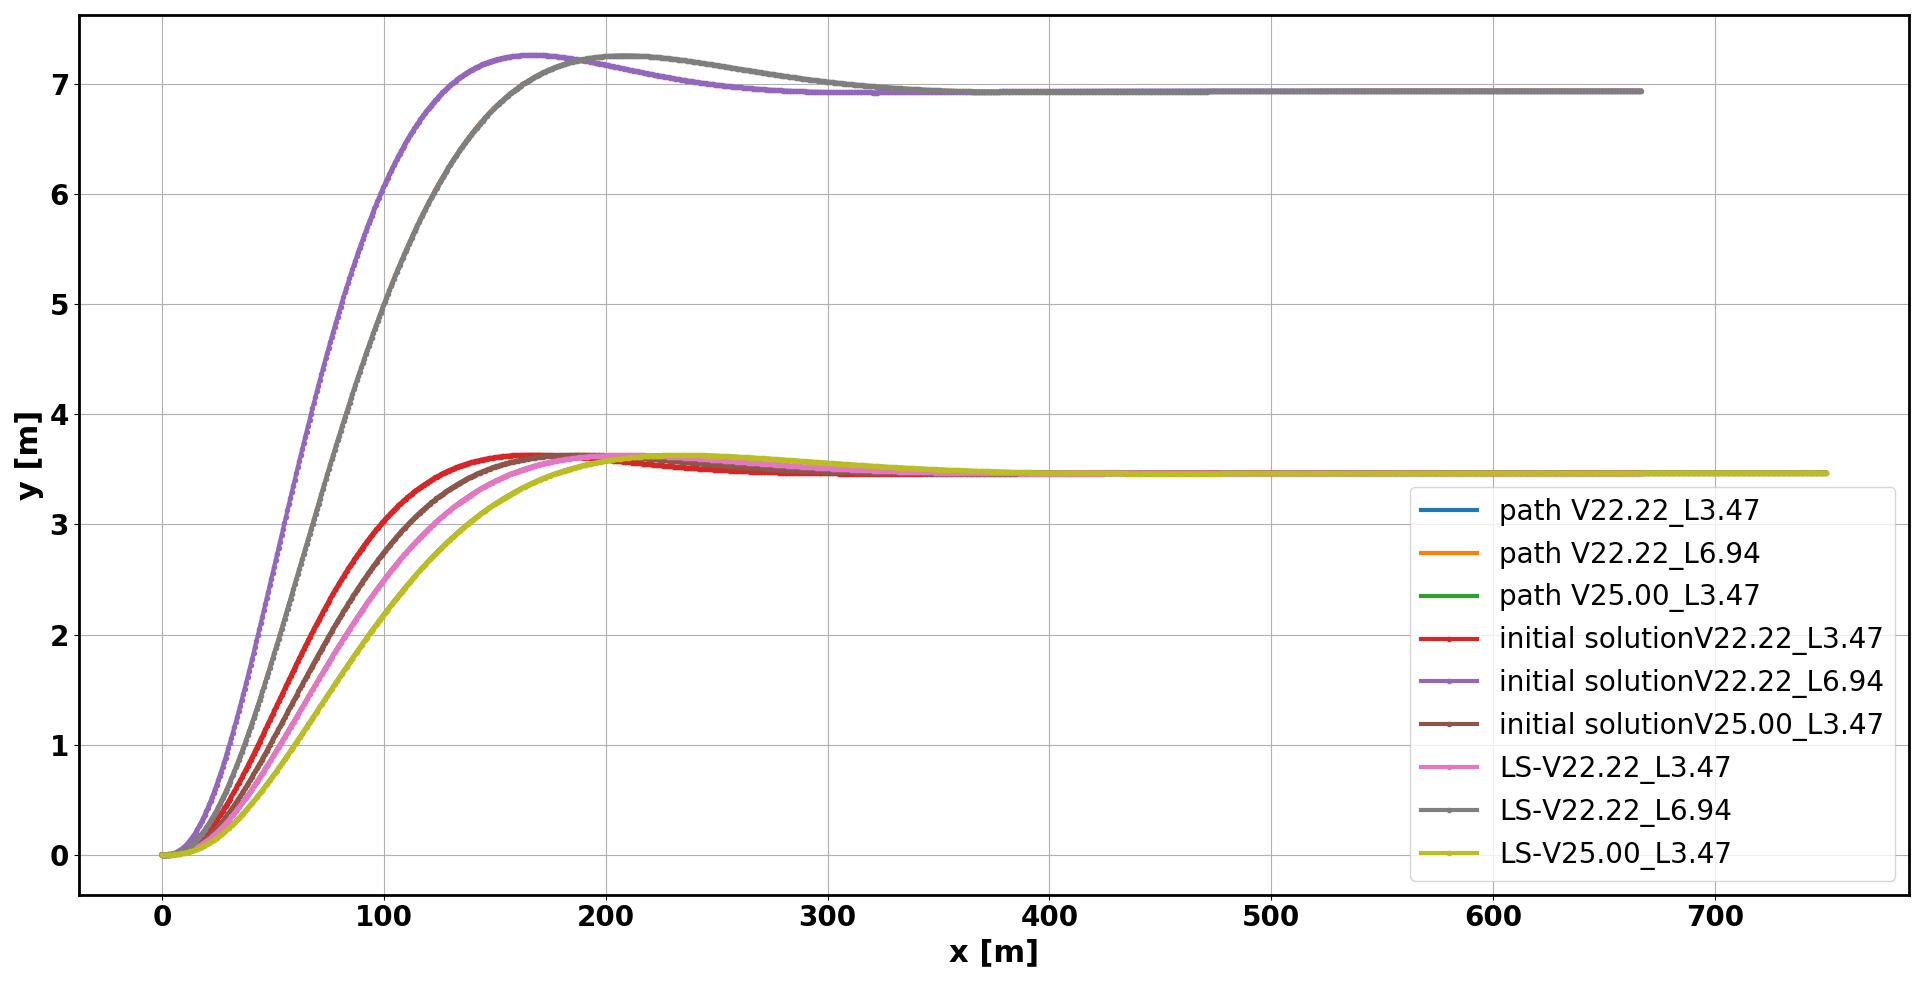
\includegraphics[width=1.0\textwidth]{3D_LP.png}
	\caption{Observed, initial and learned paths for 3 different observed lane changes generated with common underlying objective function.}
	\label{fig:3D_learned_path}
\end{figure}
 
The progress towards convergence over the iterations is showed in Figure \ref{fig:3D_conv}. Convergence is reached in $25$ iterations.

\begin{figure}[h!]
	\centering
	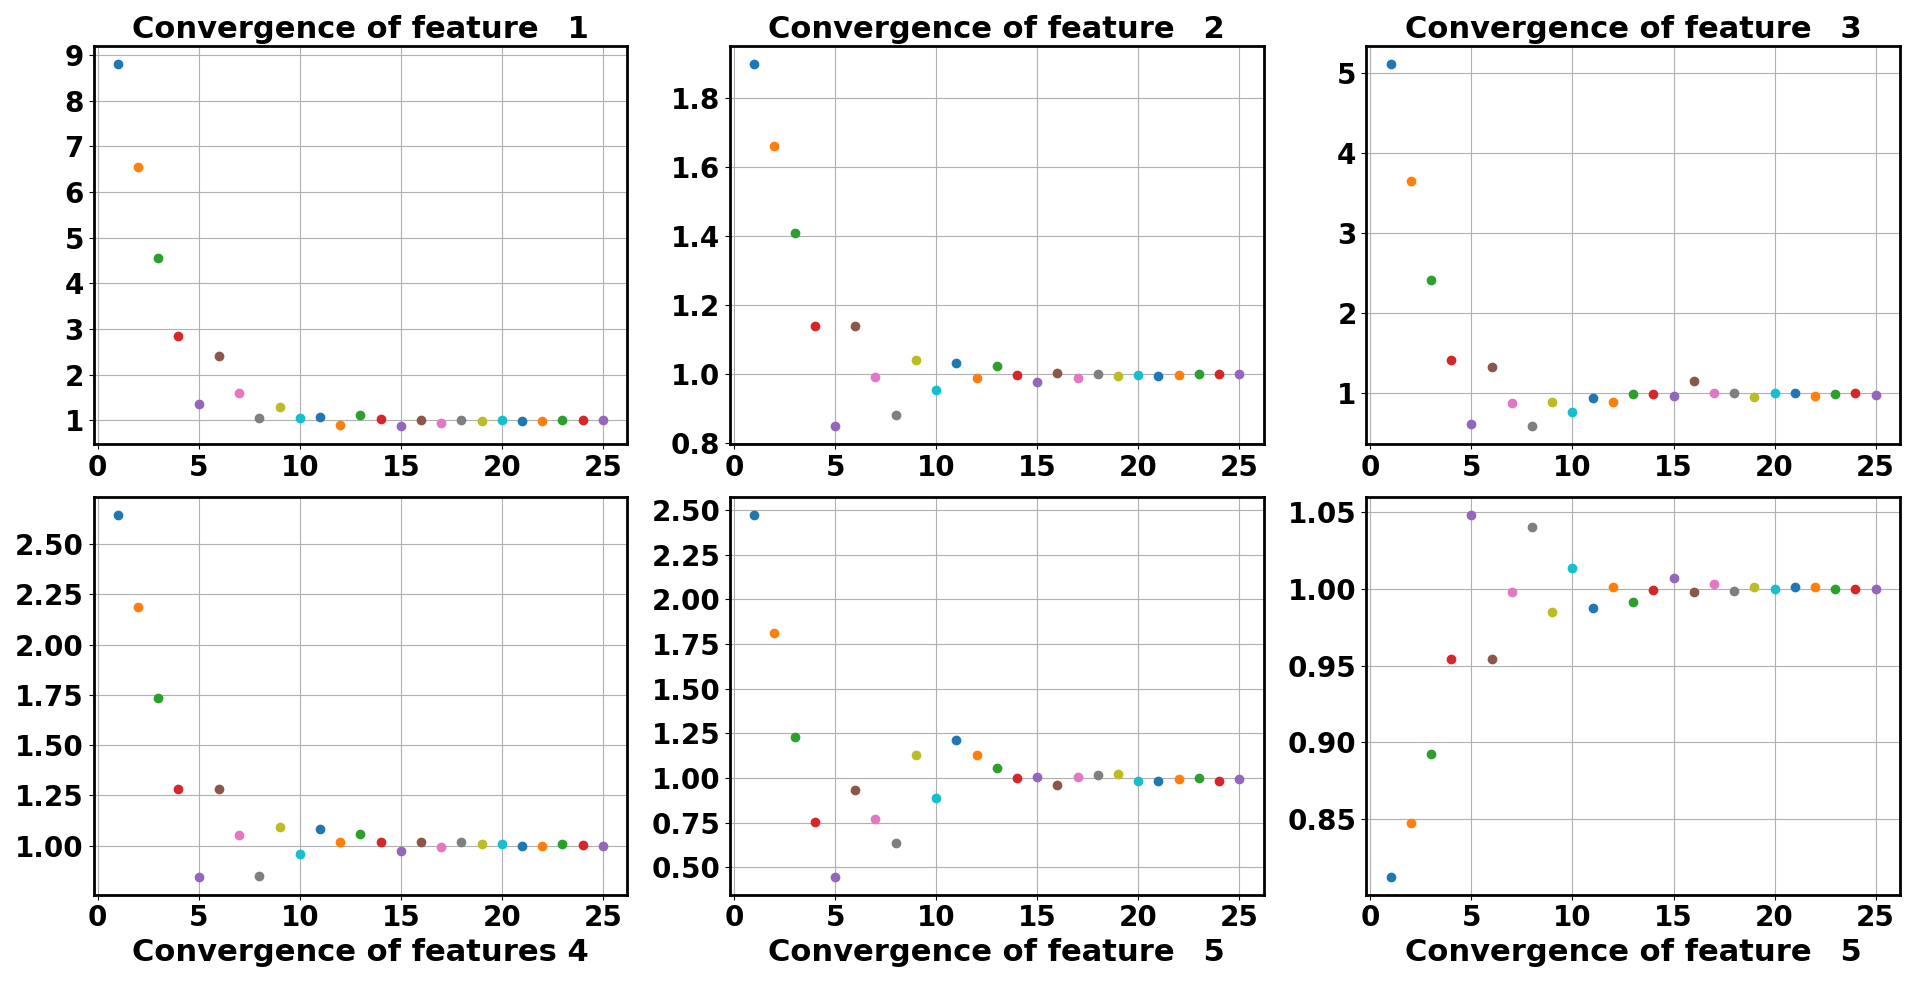
\includegraphics[width=1.0\textwidth]{3D_conv.png}
	\caption{The evolvement of the average $\bm{f}_{rel}$ over the learning iterations.}
	\label{fig:3D_conv}
\end{figure}

Figure \ref{fig:3D_w} gives a view of how the learned weighting factors change over the iterations for the different features. The weighting factors in these graphs differ with the ones shown at the beginning of this section by a scaling factor $\frac{5.0}{\theta_2}$. Both these weighting factors will generate the exact same lane change when used in the objective of Eq. (\ref{opt:basic_opti_w}). During the learning process this degree of freedom can be removed by fixing the second weight equal to $5.000$. Convergence is reached after $59$ iterations and following weighting factors are outputted $\bigl[ \begin{smallmatrix} 15.143,&5.000,&3.222,&6.016,&3.880,&2.007\end{smallmatrix}\bigr]$ where the lateral weighting factors again clearly are found back. It takes the algorithm longer to find equivalent weighting factors because of the lost in the ability of the RPROP algorithm to update all the weighting factors. Therefore the scaling degree of freedom is retained during the rest of this thesis. \\

 
\begin{figure}[h!]
	\centering
	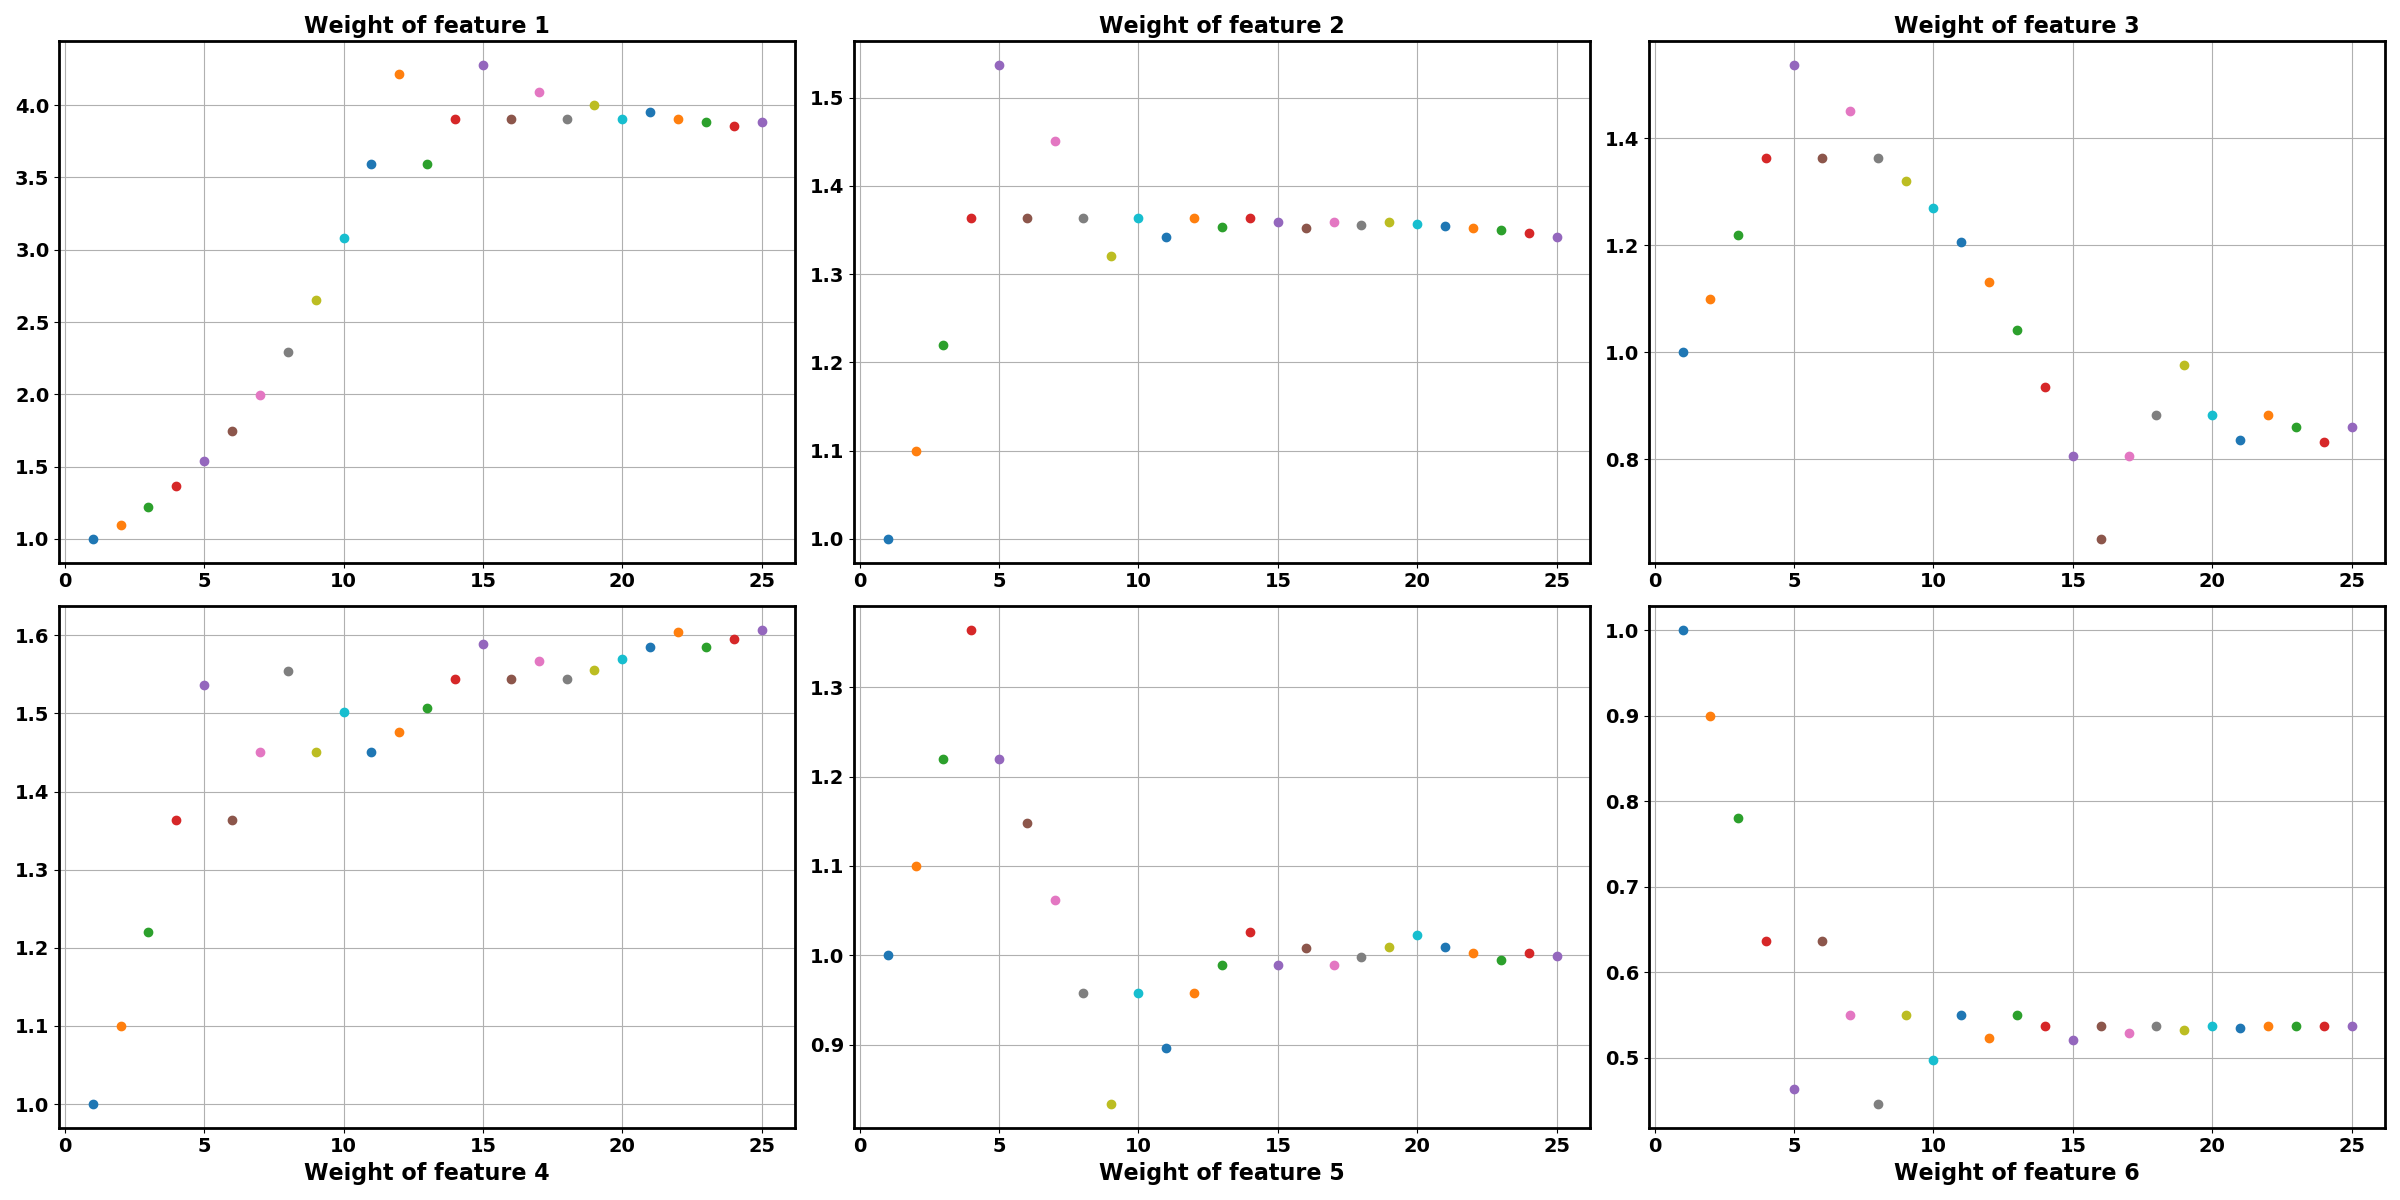
\includegraphics[width=1.0\textwidth]{3D_w.png}
	\caption{The different outputted weighting factors over the learning iterations.}
	\label{fig:3D_w}
\end{figure}

\subsection{Conflict method}\label{s:conflict_method}
 The second method proposed to learn simultaneous of multiple datasets, is the conflict method. Its main idea is to only update a weight if the gradient, as given by Eq. (\ref{eq:new}), of the different individual datasets point all in the same direction. If there are individual gradients with conflicting signs, the update direction is ambiguous and the concerning weight is not updated. The updating will be resumed when the conflict is solved by updating the other weighting factors. Solving conflicts is possible because the features are not independent of each other. Figure \ref{fig:conflict} shows how the conflict check is integrated together with the RPROP algorithm in the 'update weighting factors' box in the basic learning flow of Figure \ref{fig:basic learning}. The blue boxes serve as output ports.\\
 
  \begin{figure}[h!]
 	\centering
 	\includegraphics[width=1.1\textwidth]{conflict.png}
 	\caption{Flow of the conflict method as part of the basic flow diagram of Figure \ref{fig:basic learning}}
 	\label{fig:conflict}
 \end{figure}

Depending if the previous case was 'RPROP case 2' and the sign difference between the current and previous gradient, three distinct RPROP cases can be identified which outputs the new update value, delta weighting factors ($dw$) and the exception value as discussed in section \ref{s:RPROP}. Inside the conflict block, it is checked if all the signs of the current gradients are consistent. This boils down to verifying on which entry in the $m$ different gradients there is a sign difference. Here is $m$ the amount of observations and an individual gradient is calculated as  $\bm{F}_{obs,i} - \bm{F}(\bm{r}_{expected,i})$ with $m \in \mathbb{N}_{[1\dots ND]}$. \\ 

If there is a sign difference, this means that for one dataset the learned feature value is higher than the observed one and the corresponding weight should be increased (negative gradient) and for at least one other dataset, the corresponding weight should be decreased (positive gradient). For such a case the conflict test will give rise to a positive conflict value. If there is no conflict there will also be unity in the decision of the RPROP case, because no conflict was spotted in the gradients during the previous iteration. When a conflict is resolved, the next case will be automatically equal to RPROP case 3 because no decision can be made to either increase or decrease the update value. The convergence criteria used stays the same as discussed in \ref{s:averaging_method} but now an additional criteria is added that there should still be improvement possible. This means that it should be possible to update a weight in a direction that benefits every dataset.\\

The learning algorithm is applied on the same three datasets as discussed in section \ref{s:averaging_method} and uses as initial guess of the weighting factors an all-one vector. The resulting weighs found after $32$ iterations are  $\bigl[ \begin{smallmatrix} 14.283,&5.000,&3.114,&5.979,&3.645,&2.000\end{smallmatrix}\bigr]$. The learning algorithm stopped because no update of the weighting factors could be done without ambiguity. It can be concluded that the lateral weighting factors are found back. The $\bm{f}_{rel}$ of the individual datasets can be seen in table \ref{tab:in_conflict}. It is shown in the table that there is a good match between the learned feature vectors and the individual data feature vectors. Figure \ref{fig:3D_conv_conflict} presents the convergence of the $\bm{f}_{rel}$ vector of dataset $V_0:22.22\hspace{1mm}\frac{m}{s},\hspace{1mm} L:3.47\hspace{1mm}m$. The individual convergence plots for the other datasets are very similar.\\

\begin{table}[h!]
	\centering
	\begin{tabular}{@{}llllr@{}} \toprule
		$\bm{f}_{rel}$    & V022.22 - L3.47 & V022.22 - L6.94 & V025.00 - L3.47\\ \midrule
		Nr.1       		  &0.9939       & 0.9913 	    & 1.0003 		\\
		Nr.2              & 1.0003       & 0.9993       & 1.0002       \\
		Nr.3              & 0.9911       & 0.9868       & 1.0032      \\
		Nr.4              & 1.0016       & 0.9999       & 1.0014       \\
		Nr.5              & 1.0009       & 0.9985       & 0.9941       \\
		Nr.6              & 0.9998       & 1.0001       & 0.9998       \\ \bottomrule
	\end{tabular}
	\caption{This table shows the $\bm{f_{rel}}$ for each individual dataset at convergence using the conflict method.}
	\label{tab:in_conflict}
\end{table} 


\begin{figure}[h!]
	\centering
	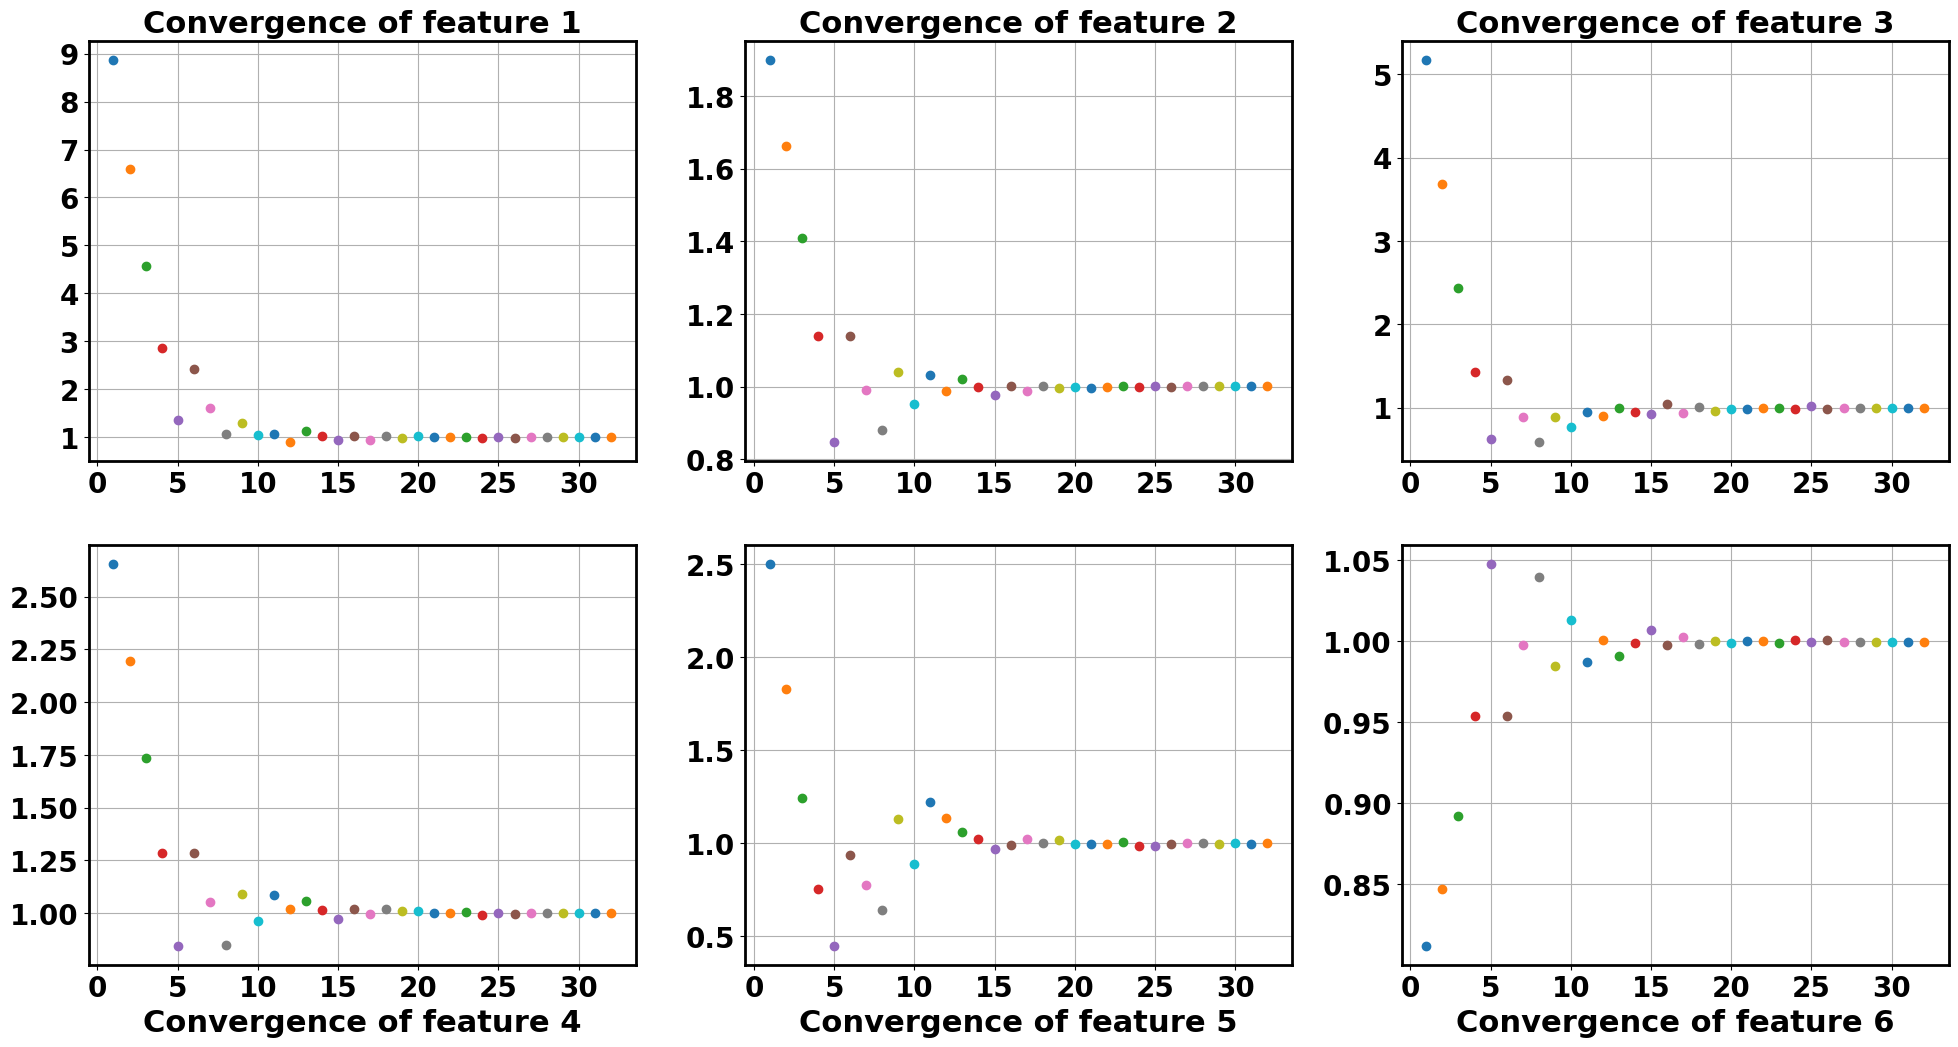
\includegraphics[width=1.0\textwidth]{3D_conv_conflict.png}
	\caption{The evolvement of $\bm{f}_{rel}$ of dataset  $V_0:22.22\hspace{1mm}\frac{m}{s},\hspace{1mm} L:3.47\hspace{1mm}m$ over the learning iterations.}
	\label{fig:3D_conv_conflict}
\end{figure}

As can be seen in table \ref{tab:in_conflict} and Figure \ref{fig:3D_conv_conflict} the conflict method is capable to give an adequate convergence towards the observed features. As is demonstrated in section \ref{s:averaging_method} when the feature values match there is also a good match between the learned and demonstrated kinematic signals.\\

The algorithm was stopped because no improvement could be realized anymore. It could be hypothesized that if real driver data is used where the human driver is less consistent in producing observations that resemble its underlying objective, the algorithm is stopped earlier. This will naturally constrict the algorithm in its feature matching accuracy due to no available direction of improvement. This can already be seen when more datasets are used in the conflict method e.g. 7 datasets. The algorithm stops then at $25$ iterations because it reached earlier a point of no improvement. The learned weighting factors for 7 datasets are $\bigl[ \begin{smallmatrix} 14.785,&5.000,&3.223,&5.968,&3.770,&2.000\end{smallmatrix}\bigr]$. \\
Figure \ref{fig:acc_conflict} gives the averaged error that each individual $\bm{f}_{rel,i}$ vector makes with respect to convergence to one for the three important lateral features. The three important lateral features shown in Figure \ref{fig:acc_conflict} are respectively the remaining lateral distance, lateral acceleration and lateral jerk. $ND$ stands for number of datasets used.

\begin{figure}[h!]
	\centering
	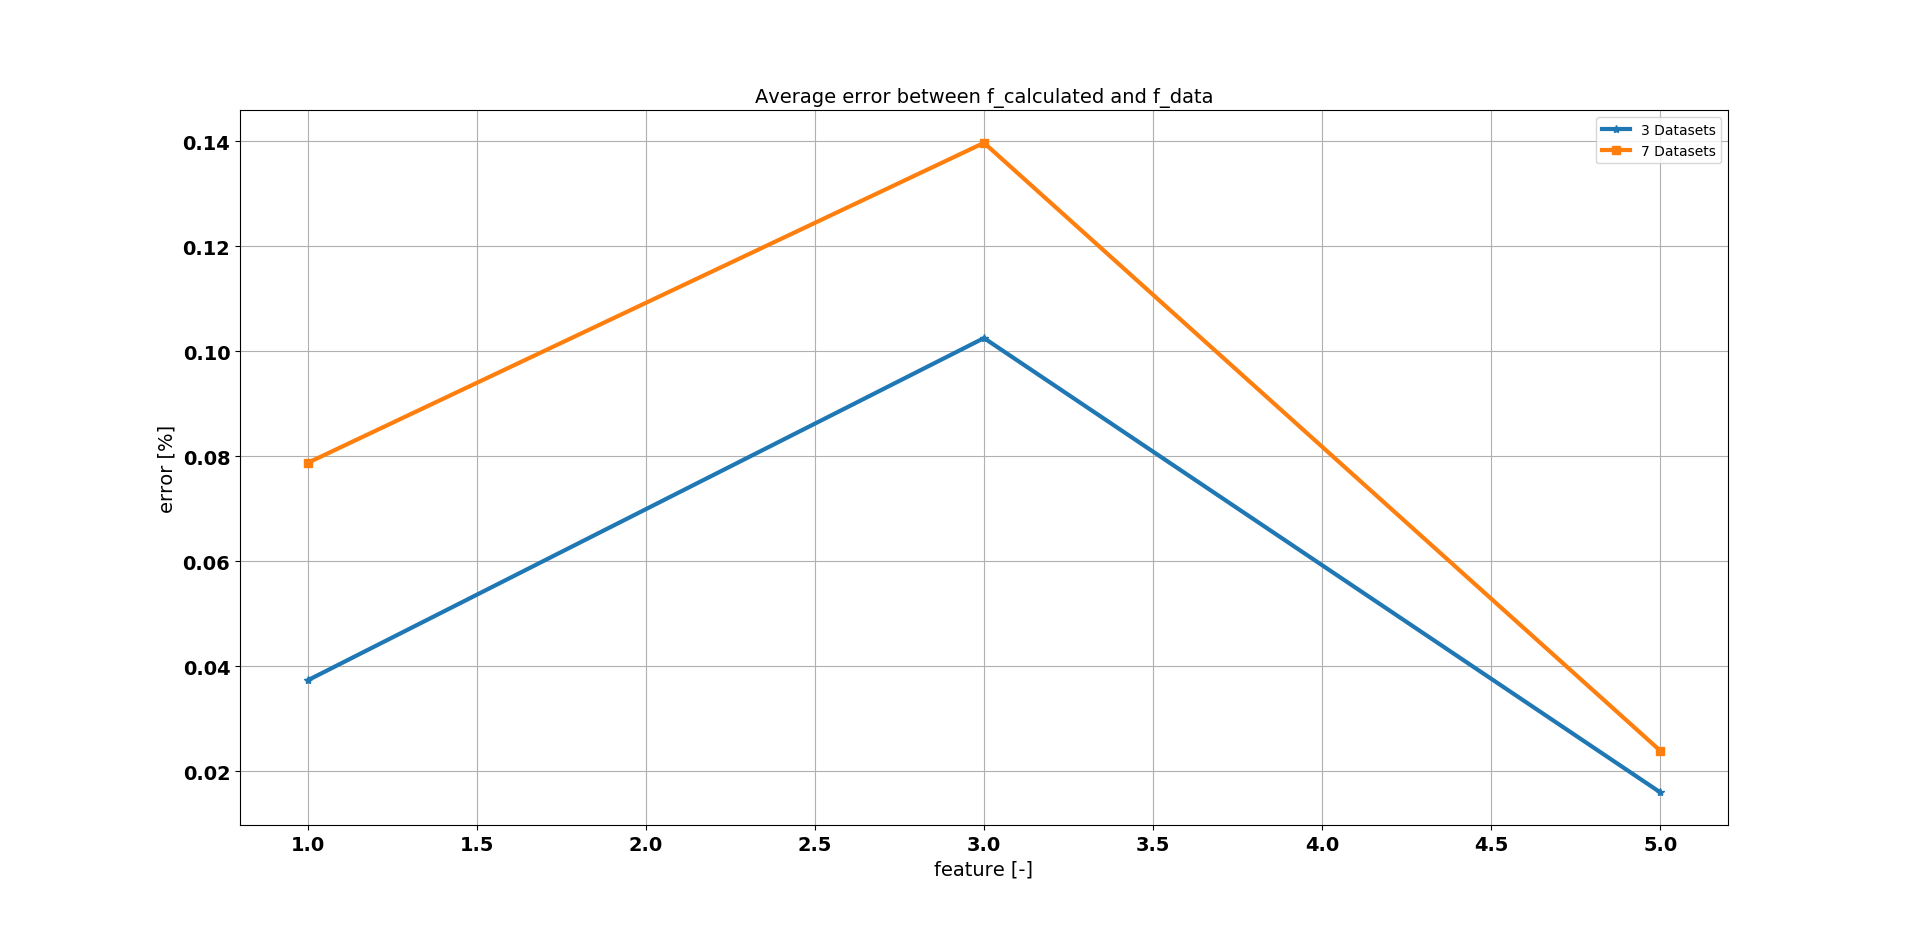
\includegraphics[width=1.1\textwidth]{acc_conflict.png}
	\caption{This figure shows the averaged, relative error given by $\frac{100\cdot\sum_{n=1}^{ND}|1-f_{rel,i}|}{ND}$ of the matching of the feature values for the three lateral features. (3 datasets: blue, 7 datasets: orange)}
	\label{fig:acc_conflict}
\end{figure}

Figure \ref{fig:acc_conflict} shows that the prematurely stop of learning with 7 datasets in comparison with 3 datasets gives an slightly higher error in the match of feature values of the individual datasets.    
 
\subsection{Comparison of methods}\label{s:comparison of methods}
In this section a comparison is made between the averaging and conflict method of combining multiple datasets. Figure \ref{fig:acc_comp} shows that the averaging method learns weighting factors that can better explain the individual data feature vectors of the different datasets. Therefore this will be the method further used during this thesis.

\begin{figure}[h!]
	\centering
	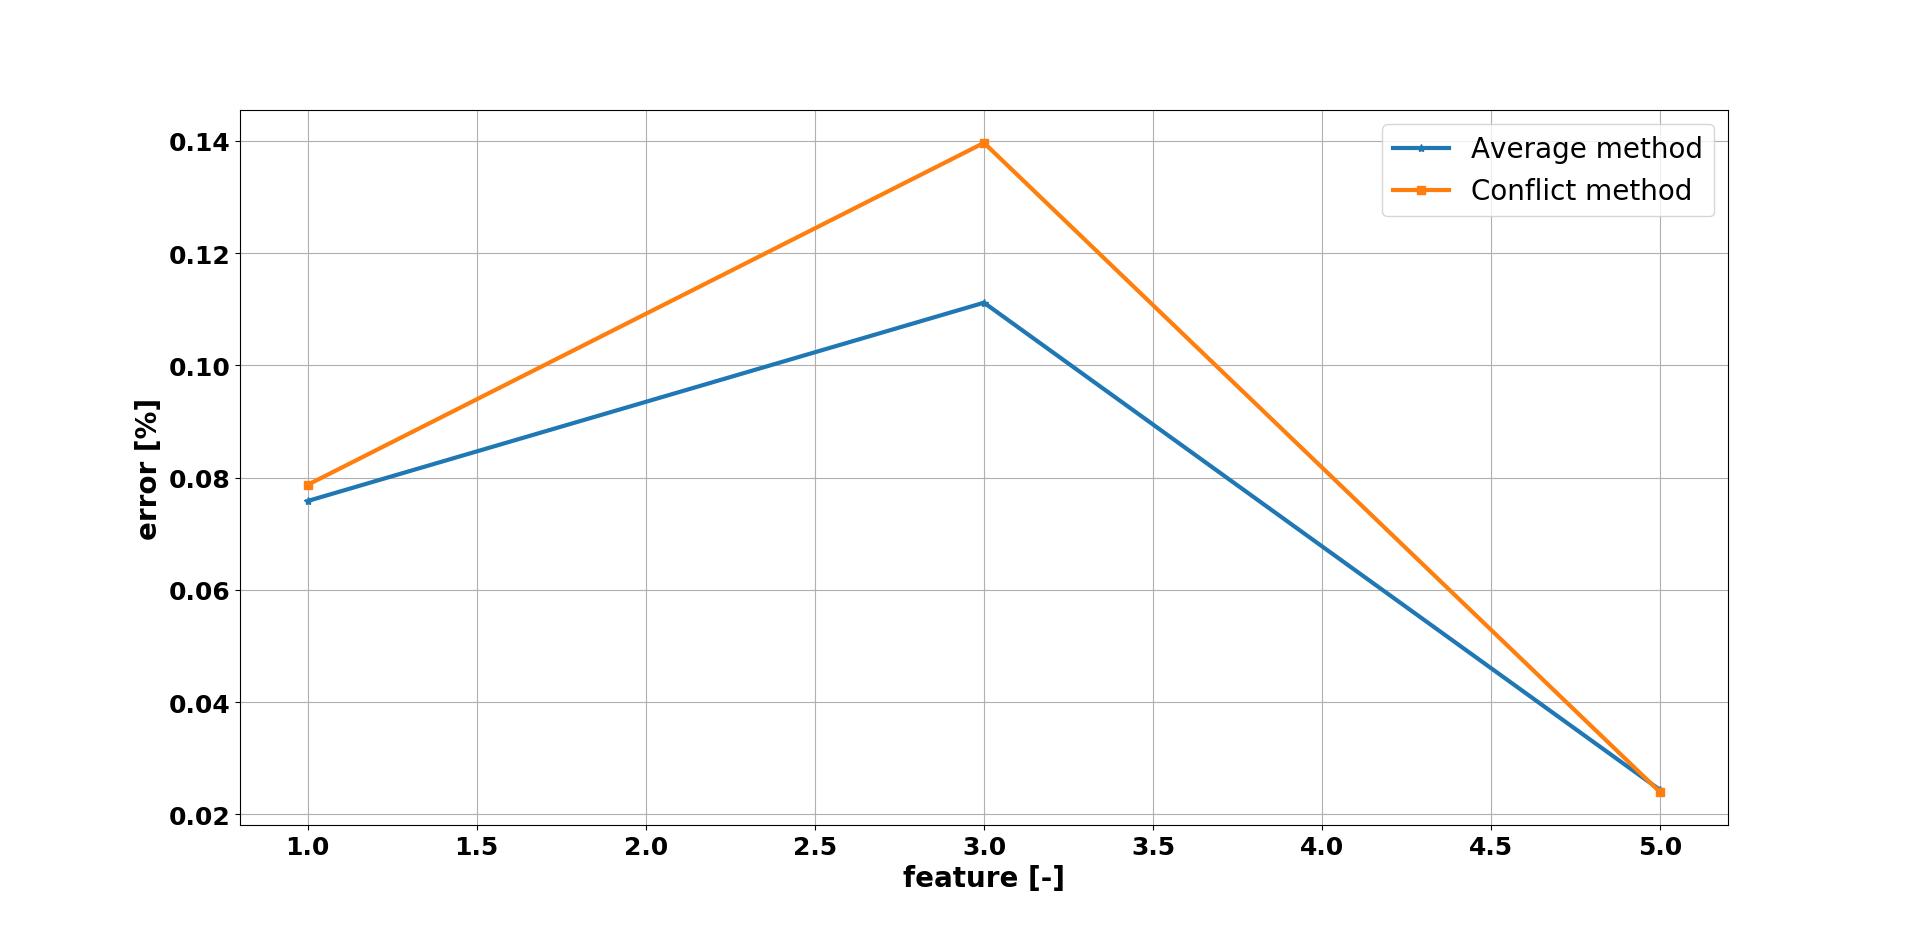
\includegraphics[width=1.0\textwidth]{acc_comp.png}
	\caption{This figure shows the averaged, relative error given by $\frac{100\cdot\sum_{n=1}^{ND}|1-f_{rel,i}|}{ND}$ of the matching of the feature values of the three lateral features. (Averaging method: blue, conflict method: orange)}
	\label{fig:acc_comp}
\end{figure}

\newpage
 \section{Conclusion} \label{s:conclusion_cha4}
In this chapter the implementation of learning from ideal data was analysed. Data is considered ideal when it is produced with the same vehicle model as is used during the learning loop which calls the optimization Eq. (\ref{opt:basic_opti_w}). During this chapter first the non-linear bicycle model was discussed and its used parameters are presented in table \ref{table:vehicel_model_param}. Next a step by step building up of the learning algorithm is shown. It is displayed how the ideal data is generated and validated. Out of this it followed that the choice of number of control points was set on $1000$ and the time limit on $30 \hspace{1mm}s$. Afterwards the learning results were discussed and the conflict and averaging method were compared. It was concluded that for a lane change maneuver it is only important to learn the lateral weighting factors accurately in order to explain the observed data. Feature matching was also accomplished for the longitudinal features but there was a boundary on the accuracy due to the small longitudinal feature values attained during a lane change. Contrary to the lateral weighting factors, the longitudinal chosen weighting factors were not accurately found back. Because the conflict method gives for the same amount of datasets a slightly larger error on the ability to explain the individual feature values and because of the hypothesis that this method will behave worse when used with real driver data, the averaging method is chosen to be further used in this thesis. The estimate of the gradient $\pdv{\bm{F}_{diff}}{\bm{\theta}}$ by $\bm{F}_{obs} - \bm{F}(\bm{r}_{expected})$ was found adequate in order to match the learned and observed feature values.


%Dit is gemachtigd omdat men hier de omgeving wil scannen voor een feasible pad --> dit wordt trager gedaan dan de tracking.(tracking zal gebruik maken van een meer complex model) Path planning ligt focus vooral op de omgeving.
%Hoe zal de methode gevalideerd worden? Leg de twee methodes uit: code generatie en kijken of de wegings factoren terug gevonden kunnen worden? Mappen de feature values met de values van het geobserveerde pad? --> is het doel dat gevolgd probeert te worden haalbaar? 

%Vermeld afleiding van algortihm. Leg uit in Thesis hoe komt aan gradient die gebruikt. Zie papers: Ziebart et al and Kretzschmar et al.
%
%Modeleer een andere bestuurder. Can try to reproduce a data set with a change of parameters which represents a different driver. Can check that the learned model is also different. Hiermee aantonen dat er ook echt andere wegingsfactoren worden gegenereerd en dat de specifieke driving characteristics worden meegenomen.
%
%Ligt een tipje van de sluier op : hoe zal de data gegenereerd worden? 

%
%Maak een vermelding dat men het menselijke gedrag van het geleerde model kan nagaan met een Turing test.\\
%
%Maak een plotje zoals paper Learning to Predict Trajectories of Cooperatively Navigating Agents --> feature variance afwijking en average error. (zelfde plotjes als al de papers)\\
%
%Schrijf een paragraaf over hoe de data gegenereerd wordt. %
%
%Kan vermelding maken dat in deze thesis de features zijn gekozen met de hand --> men kan proberen om de features ook te leren van date (Characterizing Driving Styles with Deep Learning)
% Try to validate the chosen features with looking at the sensitivity.

%%Afleiding van exponentiël functie zie paper: Feature-based prediction of trajectories for socially compliant navigation (foto) --> weighting factors are lagrange coefficients.


%\section{Tables}
%Tables are used to present data neatly arranged. A table is normally
%not a spreadsheet! Compare \tref{tab:wrong} en \tref{tab:ok}: which table do
%you prefer?
%
%\begin{table}
%  \centering
%  \begin{tabular}{||l|lr||} \hline
%    gnats     & gram      & \$13.65 \\ \cline{2-3}
%              & each      & .01 \\ \hline
%    gnu       & stuffed   & 92.50 \\ \cline{1-1} \cline{3-3}
%    emu       &           & 33.33 \\ \hline
%    armadillo & frozen    & 8.99 \\ \hline
%  \end{tabular}
%  \caption{A table with the wrong layout.}
%  \label{tab:wrong}
%\end{table}
%
%\begin{table}
%  \centering
%  \begin{tabular}{@{}llr@{}} \toprule
%    \multicolumn{2}{c}{Item} \\ \cmidrule(r){1-2}
%    Animal    & Description & Price (\$)\\ \midrule
%    Gnat      & per gram    & 13.65 \\
%              & each        & 0.01 \\
%    Gnu       & stuffed     & 92.50 \\
%    Emu       & stuffed     & 33.33 \\
%    Armadillo & frozen      & 8.99 \\ \bottomrule
%  \end{tabular}
%  \caption{A table with the correct layout.}
%  \label{tab:ok}
%\end{table}


%%% Local Variables: 
%%% mode: latex
%%% TeX-master: "thesis"
%%% End: 
